\documentclass{svjour3}                     % onecolumn (standard format)
%\documentclass[smallcondensed]{svjour3}     % onecolumn (ditto)
% \documentclass[smallextended]{svjour3}       % onecolumn (second format)
% \documentclass[twocolumn]{svjour3}          % twocolumn
%
\smartqed  % flush right qed marks, e.g. at end of proof
%
\usepackage{graphicx}
\usepackage{amsmath,amssymb,amsfonts}

\journalname{Archive of Applied Mechanics}
%
\begin{document}

\title{Revisit to the theoretical analysis of a classical piezoelectric vibration energy harvester }
\titlerunning{Model and Analysis of PVEH}        % if too long for running head

\author{Maoying Zhou         \and
        Huijun Zhao %etc.
}

%\authorrunning{Short form of author list} % if too long for running head

\institute{Maoying Zhou \and Huijun Zhao \at
              School of Mechanical Engineering, Hangzhou Dianzi University \\
              \email{myzhou@hdu.edu.cn}           %  \\
}

\date{Received: date / Accepted: date}
% The correct dates will be entered by the editor


\maketitle

\begin{abstract}
In this paper, we investigate the classical problem for a classical piezoelectric vibration energy harvester. Exact theoretical solution to the problem is derived and compared to the solutions proposed in the literature. Asymptotic expansions of the solution is explored in the hope of finding a plausible simpler approximation of the solution and corresponding output performance measures. Dependence of the output performance measures upon the electromechanical coupling factor is therefore studied. Some tips are then provided for the design of piezoelectric energy harvester.

\keywords{Piezoelectric vibration energy harvesting  \and Modal expansion \and Harmonic balance \and Asymptotic expansion}
% \PACS{PACS code1 \and PACS code2 \and more}
% \subclass{MSC code1 \and MSC code2 \and more}
\end{abstract}

\section{Introduction}

The soaring development of wireless sensor networks (WSNs) and Internet of Things (IoTs) in the past decades has intrigued the research into sustainable and renewable energy sources for low-power electronics. The primary research goal is to partially or even fully replace currently used battery power or utility wall power, which are generally expensive, inconvenient, and sometimes impossible. To this end, much attention has been paid to energy harvesters, which convert the available energy in the ambient environment into usable electricity. A number of principles, mechanisms, and implementations of energy harvesters have been put forward since their first appearance in the 1990s, \cite{beeby2006energy,anton2007review,zhou2018review,safaei2019review} among which piezoelectric vibration energy harvesters (PVEHs) have gained the most widespread research popularity. 

PVEHs are typically composite structures made up of some piezoelectric elements and vibration transduction mechanisms. They are generally attached to the host structures and undergo forced vibration. With the help of the vibration transduction mechanisms, the piezoelectric elements are excited in the desired vibration modes and generate electrical outputs due to direct piezoelectric effect. A majority of PVEHs work in resonance, in the sense that the maximum output power for an externally connected pure resistance is achieved when the base excitation frequency matches that of the PVEH. \cite{roundy2003study} To understand the operation principles and guide the performance optimization, researchers have proposed different mathematical models for PVEHs. 

A most direct and simple approach is to use the single-degree-of-freedom (SDOF) approximation, in which the electrical domain and the mechanical domain are using SDOF resonator models respectively. Besides, the electromechanical coupling between these two domains is represented by a constant coefficient. \cite{roundy2003study,dutoit2005design} This lumped-parameter model provides fruitful insights into the mechanism and dynamics behind the energy harvesting process and has been employed in the performance improvement and optimization of PVEHs. \cite{stephen2006energy,cottone2009nonlinear} However, it has been shown that this model only applies to one vibration mode and exhibits considerable inaccuracy in some circumstances. \cite{erturk2008mechanical}

A different yet improved approach is to resort to the Rayleigh-Ritz method. In this approach, electromechanical model of the PVEHs in the variational form is established based on the generalized Hamilton's principle, \cite{crandall1968dynamics} which is then discretized to a finite-dimension matrix-form state space model using the Rayleigh-Ritz method. \cite{hagood1990modelling} This approach can easily be modified to admit finite element analysis and be appropriate for numerical computation. Although experimentally validated and theoretically refined, \cite{sodano2004estimation,lu2003modeling,chen2006analytical,ajitsaria2007modeling} this kind of method does not reflect the resonance phenomenon and the related modal expansions. 

To address the issues, a formal expansion method is developed based on the theory of functional analysis. \cite{kreyszig1978introductory} Mechanical part of the PVEH is modeled using a partial differential equation with the help of Euler-Bernoulli assumptions, while the electrical part is described with an ordinary differential equation provided that a pure resistive load is connected to the PVEH. \cite{erturk2008distributed} Using the eigenfunctions of a cantilever beam as the basis functions, the derived system of equations is formally expanded to obtain an infinite series of sub-systems of ordinary differential equations. This method has been validated and successfully applied to PVEHs with end mass \cite{erturk2009experimentally}, to optimize the electrode coverage \cite{erturk2009effect} and some other circumstances. However, it includes infinite terms of expansion and inevitably suffers from the truncation error during numerical calculation. Besides, the basis functions adopted in the above method do not take into account the piezoelectric effect and therefore fails to capture the accurate mode shape of the PVEH theoretically.

Here in this contribution, we focus on an exact analytical model classical PVEHs. Based on the Euler-Bernoulli beam model and the linear piezoelectric relations, electromechanical model of the energy harvester is established, and then converted to a boundary value problem of ordinary differential equations using the harmonic balance method. Closed-form solution of the relative displacement function of the cantilever beam as well as the output performance measures is analyzed and numerically investigated. Asymptotic expansions of the relative displacement function are calculated to obtain approximate expressions for the output index and the related output performance measures. Tips are then provided in terms of the structure design and performance optimization of piezoelectric energy harvesters. 


\section{Mathematical model for a typical PVEH}

As shown in Figure~\ref{fig:fig_pveh}, a typical PVEH is composed of a piezoelectric composite cantilever beam attached to a host structure. For the sake of simplicity, a pure resistor is generally connected to the piezoelectric elements to represent practical electrical loads. Actually, this is a little bit of an oversimplification in the sense that no external capcitors and inductors are included in the system and that extra interface circuits and power management circuits are usually needed to achieve a better energy harvesting performance. \cite{shu2006analysis,shu2007improved,qiu2009comparison} 

\begin{figure*}[!htbp]
    \centering
    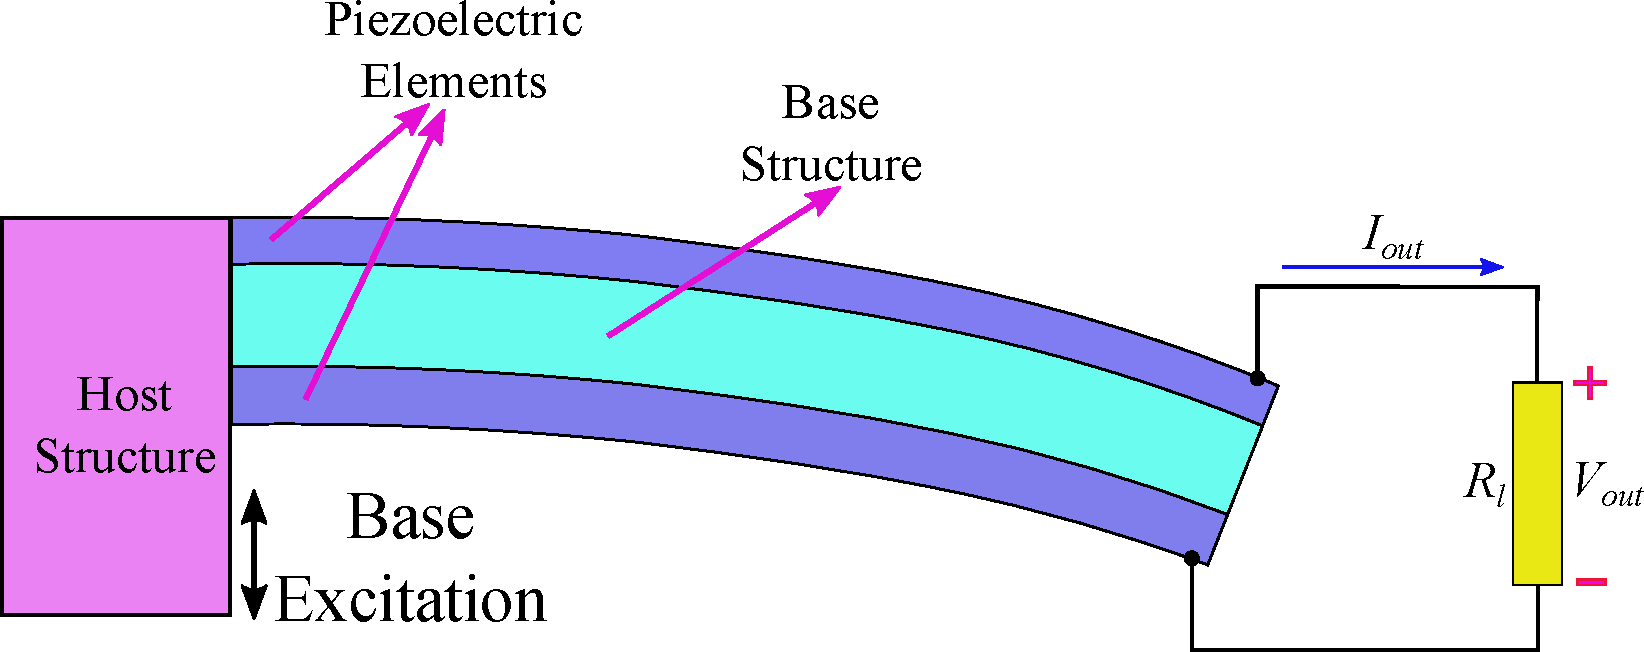
\includegraphics[width=0.8\textwidth]{./img_eig_asy/fig_pveh}
    \caption{Schematic diagram of a typical PVEH. The bimorph structure of the PVEH is just for demonstration. Actually, many different configurations can be adopted. }
    \label{fig:fig_pveh}
\end{figure*}

Based on the Euler-Bernoulli assumptions, mechanical response of the piezoelectric composite beam is described by the classical equations
\begin{equation}
    B_p \frac{\partial^4 w(x,t)}{\partial x^4} + m_p \frac{\partial^2 w(x,t)}{\partial t^2} = 0,
\end{equation}
where $w(x,t)$ denotes the displacement function of the composite beam, $B_p$ is the equivalent bending stiffness and $m_p$ is the line mass density of the piezoelectric cantilever beam. If the piezoelectric elements attached to the cantilever beam is connected to an external electrical load $R_l$, we have 
\begin{equation}
    \frac{d Q_p(t)}{d t} + \frac{V_p(t)}{R_l} = 0,
\end{equation}
in which $Q_p(t)$ is the accumulated charge on the electrodes, and $V_p(t)$ is the voltage output across the load resistor $R_l$. Deriving from the classic piezoelectric constitutive relations, we have 
\begin{equation}
    \left\{\begin{aligned}
        M_p(x,t) &= B_p \frac{\partial^2 w(x,t)}{\partial x^2} - e_p V_p(t), \\
        Q_p(x,t) &= e_p \left.\left[ \frac{\partial w(x,t)}{\partial x} \right]\right|_0^{l_p} + C_p V_p(t),
    \end{aligned}\right.
\end{equation}
where $e_p$ is the piezoelectric coupling coefficient, $C_p$ is the equivalent internal capacitance of the piezoelectric elements, and $l_p$ is the length of the composite beam. As one end of the cantilever beam is attached to the host structure and subject to base excitation. The boundary conditions for the problems are 
\begin{equation}
    \left\{\begin{aligned}
        w(0,t) &= w_b(t), \\
        \frac{\partial w(0,t)}{\partial x} &= 0,
    \end{aligned}\right.
\end{equation}
and
\begin{equation}
    \left\{\begin{aligned}
        M_p(l_p,t) &= B_p \frac{\partial^2 w(l_p,t)}{\partial x^2} - e_p V_p(t) = 0, \\
        N_p(l_p,t) &= \frac{\partial M_p(l_p,t)}{\partial x} = B_p \frac{\partial^3 w(l_p,t)}{\partial x^3} = 0,
    \end{aligned}\right.
\end{equation}
where $w_b(t)$ is the base excitation displacement, $M_p$ and $N_p$ are the total moment and shear force in the cross section respectively. To make things simpler, the displacement function $w(x,t)$ is be decomposed as 
\begin{equation}
    w(x,t) = w_b(t) + w_{rel}(x,t),
\end{equation}
where $w_{rel}(x,t)$ is the relative displacement function of the composite beam. We are principally interested in a sinusoidal base excitation $w_b(t)$ which is given by
\begin{equation}
    w_b(t) = \eta_b e^{j \sigma_b t}
\end{equation}
where $\eta_b$ is the amplitude of base excitation, and $\sigma_b = 2 \pi f_b$ is the angular frequency of base excitation with $f_b$ being the base excitation frequency. Here we use a simplified version of complex representation of a periodical signal. The term $e^{j \sigma_b t}$ should actually be $Re\left\{e^{j \sigma_b t}\right\}$. Nevertheless, this won't cause any problem in the following text and serves to simplify the calculation process. It should be noted that the amplitude $\eta_b$ is generally a real number as we assume the base excitation always possesses zero phase angle. 

Considering the steady state response of the PVEH to base excitation $w_b(t)$, the relative displacement function $w_{rel}(x,t)$ and output voltage $V_p(t)$ can then reasonably be represented as 
\begin{equation}
    w_{rel}(x,t) = \eta_{rel}(x) e^{j \sigma_b t},\quad V_p(t) = \tilde{V}_p e^{j \sigma_b t},
\end{equation}
respectively, where $\eta_{rel}(x)$ and $\tilde{V}_p$ are complex amplitudes. In this way, the above model for the PVEH is simplified as 
\begin{subequations}
\begin{equation}
    B_p \frac{\partial^4 \eta_{rel}(x)}{\partial x^4} - m_p \sigma_b^2 \eta_{rel}(x) = m_p \sigma_b^2 \eta_{b},
    \label{eq:eq_dimensional_system_dynamics}
\end{equation}
\begin{equation}
    \eta_{rel}(0) = 0,
    \label{eq:eq_dimensional_system_bc0_disp}
\end{equation}
\begin{equation}
    \frac{\partial \eta_{rel}(0)}{\partial x} = 0,
    \label{eq:eq_dimensional_system_bc0_slope}
\end{equation}
\begin{equation}
    B_p \frac{\partial^2 \eta_{rel}(l_p)}{\partial x^2} + \frac{j \sigma_b R_l }{1 + j \sigma_b C_p R_l } e_p^2 \frac{\partial \eta_{rel}(l_p)}{\partial x} = 0, \\
    \label{eq:eq_dimensional_system_bc1_torque}
\end{equation}
\begin{equation}
    \frac{\partial^3 \eta_{rel}(l_p)}{\partial x^3} = 0.
    \label{eq:eq_dimensional_system_bc1_force}
\end{equation}
\end{subequations}
Here some discussions are to be made. Due to the existence of piezoelectric effect, the boundary conditions (\ref{eq:eq_dimensional_system_bc1_torque}) is tuned and deviates from the case of a pure elastic cantilever beam. \cite{weaver1990vibration} Hence for the related free vibration problem, the eigenvalue and eigenfunctions are different from that of a pure elastic cantilever beam, which is adopted in the work by Erturk and Inman \cite{erturk2008distributed,erturk2009experimentally}. Therefore the method used by Erturk and Inman \cite{erturk2008distributed,erturk2009experimentally} to expand the relative displacement function $\eta_{rel}(x)$ in terms of the eigenfunctions for a pure elastic cantilever beam is a formal one in the sense that the boundary conditions are not fulfilled by the eigenfunctions. Nonetheless, due to the orthogonality of the eigenfunctions, the expansion is mathematically feasible and a considerable accuracy can be achieved when the number of terms of expansion is large enough. This is not a perfect solution. We would like in the following to derive an exact solution to the steady state response.

To enhance the universality of our solution, we adopt the following dimensionless scheme
\begin{equation}
    u = \eta_{rel} / \eta_b ,\quad z = x / l_p 
\end{equation}
and therefore obtain the following dimensionless parameters
\begin{equation}
    \sigma = \sigma_b \sqrt{\frac{m_p l_p^4}{B_p}}, \quad \beta = R_l C_p \sqrt{\frac{B_p}{m_p l_p^4}}, \quad \delta = \frac{e_p^2 l_p}{C_p B_p}.
\end{equation}
Now, the above problem is converted into the following system of boundary value problem
\begin{equation}
    \left\{\begin{aligned}
        u^{\prime\prime\prime\prime} -\sigma^2 u &= \sigma^2, \\
        u(0) &= 0, \\
        u^{\prime}(0) &= 0, \\
        u^{\prime\prime}(1)  + \frac{j \beta \sigma }{1 + j \beta \sigma } \delta u^{\prime}(1) &= 0, \\
        u^{\prime\prime\prime}(1) &= 0,
    \end{aligned}\right.
    \label{eq:eq_dimensionless_system_all}
\end{equation}
where the prime denotes the derivative with respect to $z$.


\section{Theoretical analysis of the model}

The boundary value problem (\ref{eq:eq_dimensionless_system_all}) is a linear problem depending on the three dimensionless parameters $\beta$, $\sigma$, and $\delta$. Due to the presence of complex tuning terms in the boundary conditions, the solution $u(z)$ is generically a complex function. The analytical solution to this problem can be formulated as
\begin{equation}
    u(z;\delta) = A_\delta \cos{\sqrt{\sigma}z} + B_\delta \sin{\sqrt{\sigma}z} + C_\delta \cosh{\sqrt{\sigma}z} + D_\delta \sinh{\sqrt{\sigma}z} - 1.
    \label{eq:eq_disp_func_general_coeffs}
\end{equation}
Here we use the notation $u(z;\delta)$ to emphasize the dependence of the function $u(z)$ upon parameter $\delta$. In the following text, we will frequently use these two notations interchangeably unless otherwise declared. The coefficients $A_\delta$, $B_\delta$, $C_\delta$, and $D_\delta$ are then subject to the following linear system of equations:
\begin{equation}
    \left\{\begin{aligned}
        A_\delta + C_\delta &= 1, \\
        B_\delta + D_\delta &= 0, \\
        \left( - A_\delta \cos{\sqrt{\sigma}} - B_\delta \sin{\sqrt{\sigma}} + C_\delta \cosh{\sqrt{\sigma}} + D_\delta \sinh{\sqrt{\sigma}} \right) &+ \\
        \frac{j \beta \sqrt{\sigma}}{ j\sigma \beta + 1 } \delta \left( - A_\delta \sin{\sqrt{\sigma}} + B_\delta \cos{\sqrt{\sigma}} + C_\delta \sinh{\sqrt{\sigma}} + D_\delta \cosh{\sqrt{\sigma}} \right) &= 0, \\
        A_\delta \sin{\sqrt{\sigma}} - B_\delta \cos{\sqrt{\sigma}} + C_\delta \sinh{\sqrt{\sigma}} + D_\delta \cosh{\sqrt{\sigma}} &= 0.
    \end{aligned}\right.
\end{equation}
Analytically, we can directly obtain the solution to this problem as 
\begin{equation}
    \left\{\begin{aligned}
        A_\delta &= \frac{ 1 + \cos\sqrt{\sigma } \cosh\sqrt{\sigma } - \sin\sqrt{\sigma } \sinh\sqrt{\sigma} + \frac{2 j \beta \sqrt{\sigma}}{ 1+ j \beta \sigma } \delta \left( \cos\sqrt{\sigma } \sinh\sqrt{\sigma } \right)}{2 \left[ 1 + \cos\sqrt{\sigma } \cosh\sqrt{\sigma } + \frac{j \beta \sqrt{\sigma}}{ 1+ j \beta \sigma } \delta \left( \cos\sqrt{\sigma } \sinh\sqrt{\sigma } + \sin\sqrt{\sigma } \cosh\sqrt{\sigma } \right) \right]}, \\
        B_\delta &= \frac{ \cos\sqrt{\sigma } \sinh\sqrt{\sigma } + \sin\sqrt{\sigma } \cosh\sqrt{\sigma} + \frac{2 j \beta \sqrt{\sigma}}{ 1+ j \beta \sigma } \delta \left( \sin\sqrt{\sigma } \sinh\sqrt{\sigma } \right)}{2 \left[ 1 + \cos\sqrt{\sigma } \cosh\sqrt{\sigma } + \frac{j \beta \sqrt{\sigma}}{ 1+ j \beta \sigma } \delta \left( \cos\sqrt{\sigma } \sinh\sqrt{\sigma } + \sin\sqrt{\sigma } \cosh\sqrt{\sigma } \right) \right]}, \\
        C_\delta &= \frac{ 1 + \cos\sqrt{\sigma } \cosh\sqrt{\sigma } + \sin\sqrt{\sigma } \sinh\sqrt{\sigma} + \frac{2 j \beta \sqrt{\sigma}}{ 1+ j \beta \sigma } \delta \left( \sin\sqrt{\sigma } \cosh\sqrt{\sigma } \right)}{2 \left[ 1 + \cos\sqrt{\sigma } \cosh\sqrt{\sigma } + \frac{j \beta \sqrt{\sigma}}{ 1+ j \beta \sigma } \delta \left( \cos\sqrt{\sigma } \sinh\sqrt{\sigma } + \sin\sqrt{\sigma } \cosh\sqrt{\sigma } \right) \right]}, \\
        D_\delta &= \frac{ -\cos\sqrt{\sigma } \sinh\sqrt{\sigma } - \sin\sqrt{\sigma } \cosh\sqrt{\sigma} -  \frac{2 j \beta \sqrt{\sigma}}{ 1+ j \beta \sigma } \delta \left( \sin\sqrt{\sigma } \sinh\sqrt{\sigma } \right)}{2 \left[ 1 + \cos\sqrt{\sigma } \cosh\sqrt{\sigma } + \frac{j \beta \sqrt{\sigma}}{ 1+ j \beta \sigma } \delta \left( \cos\sqrt{\sigma } \sinh\sqrt{\sigma } + \sin\sqrt{\sigma } \cosh\sqrt{\sigma } \right) \right]}.
    \end{aligned}\right.
    \label{eq:eq_disp_func_coeffs_exps}
\end{equation}

Equations (\ref{eq:eq_disp_func_general_coeffs}) and (\ref{eq:eq_disp_func_coeffs_exps}) suffice to determine the analytical solution to the problem (\ref{eq:eq_dimensionless_system_all}). To validate this form of solution expressions for $u(z;\delta)$, we use the physical and mechanical parameters shown in \cite{erturk2008distributed} and calculate the dimensionless relative displacement function $u(z;\delta)$ and the corresponding normalized output voltage $| \tilde{V}_p/(\sigma_b^2 \eta_b) |$ at different base excitation frequency $f_b$ and load resistance $R_l$. The results are presented in Figure~\ref{fig:fig_sol_analytic_perf_vs_fr_mod}, where Figure~\ref{fig:fig_sol_analytic_perf_vs_fr_mod}(a) contains the results calculated by our method and Figure~\ref{fig:fig_sol_analytic_perf_vs_fr_mod}(b) is adapted from the reference \cite{erturk2008distributed}. It is seen that the two sets of results are close to each other, especially at small values of $f_b$. No obvious difference is present for the resonant frequency of the first order resonant mode. However the calculated resonant frequency for higher order resonant mode is clearly different. The third order resonant frequency is smaller than $800\ Hz$ in our model but larger than $800\ Hz$ in the model by Erturk and Inman \cite{erturk2008distributed}. Besides, the behaviors of the two solutions are different around the resonance. Our model predict a sharper peak. This could explained as follows. In the numerical calculations of our model, the grid steps for frequency can be chosen to be as small as possible. A finer calculation grid leads to a sharper resonant peak. Besides, the calculation of the model by Erturk and Inman \cite{erturk2008distributed} always involves with the truncation of the infinite expansion into finite terms, which introduces considerable error for larger values of $f_b$, especially at resonance. 

\begin{figure*}[!htbp]
    \centering
    \includegraphics[width=0.8\textwidth]{./img_eig_asy/fig_sol_analytic_perf_vs_fr_mod}
    \caption{Comparison of the currently obtained results (a) with that (b) by Erturk and Inman \cite{erturk2008distributed}.}
    \label{fig:fig_sol_analytic_perf_vs_fr_mod}
\end{figure*}


After validation, we are interested in the influence of parameter value $\delta$ upon the resulting dimensionless relative displacement function $u(z;\delta)$. According to equations (\ref{eq:eq_disp_func_general_coeffs}) and (\ref{eq:eq_disp_func_coeffs_exps}), the dimensionless relative displacement function $u(z;\delta)$ is completely determined by the three dimensionless parameters $\sigma$, $\beta$, and $\delta$. which can be interpreted as the dimensionless base excitation frequency, the dimensionless electrical resonant frequency, and the dimensionless electromechanical coupling strength for the PVEH respectively. As $\sigma$ and $\beta$ is determined by the base excitation $f_b$ and externally connected load $R_l$ respectively, only the parameter $\delta$ is fully determined by the structure itself. By taking different values of $\delta$ , we calculate the dimensionless relative displacement function $u(z;\delta)$ and plot the results in Figure~\ref{fig:fig_sol_analytic_disp_fun}.

\begin{figure*}[!htbp]
    \centering
    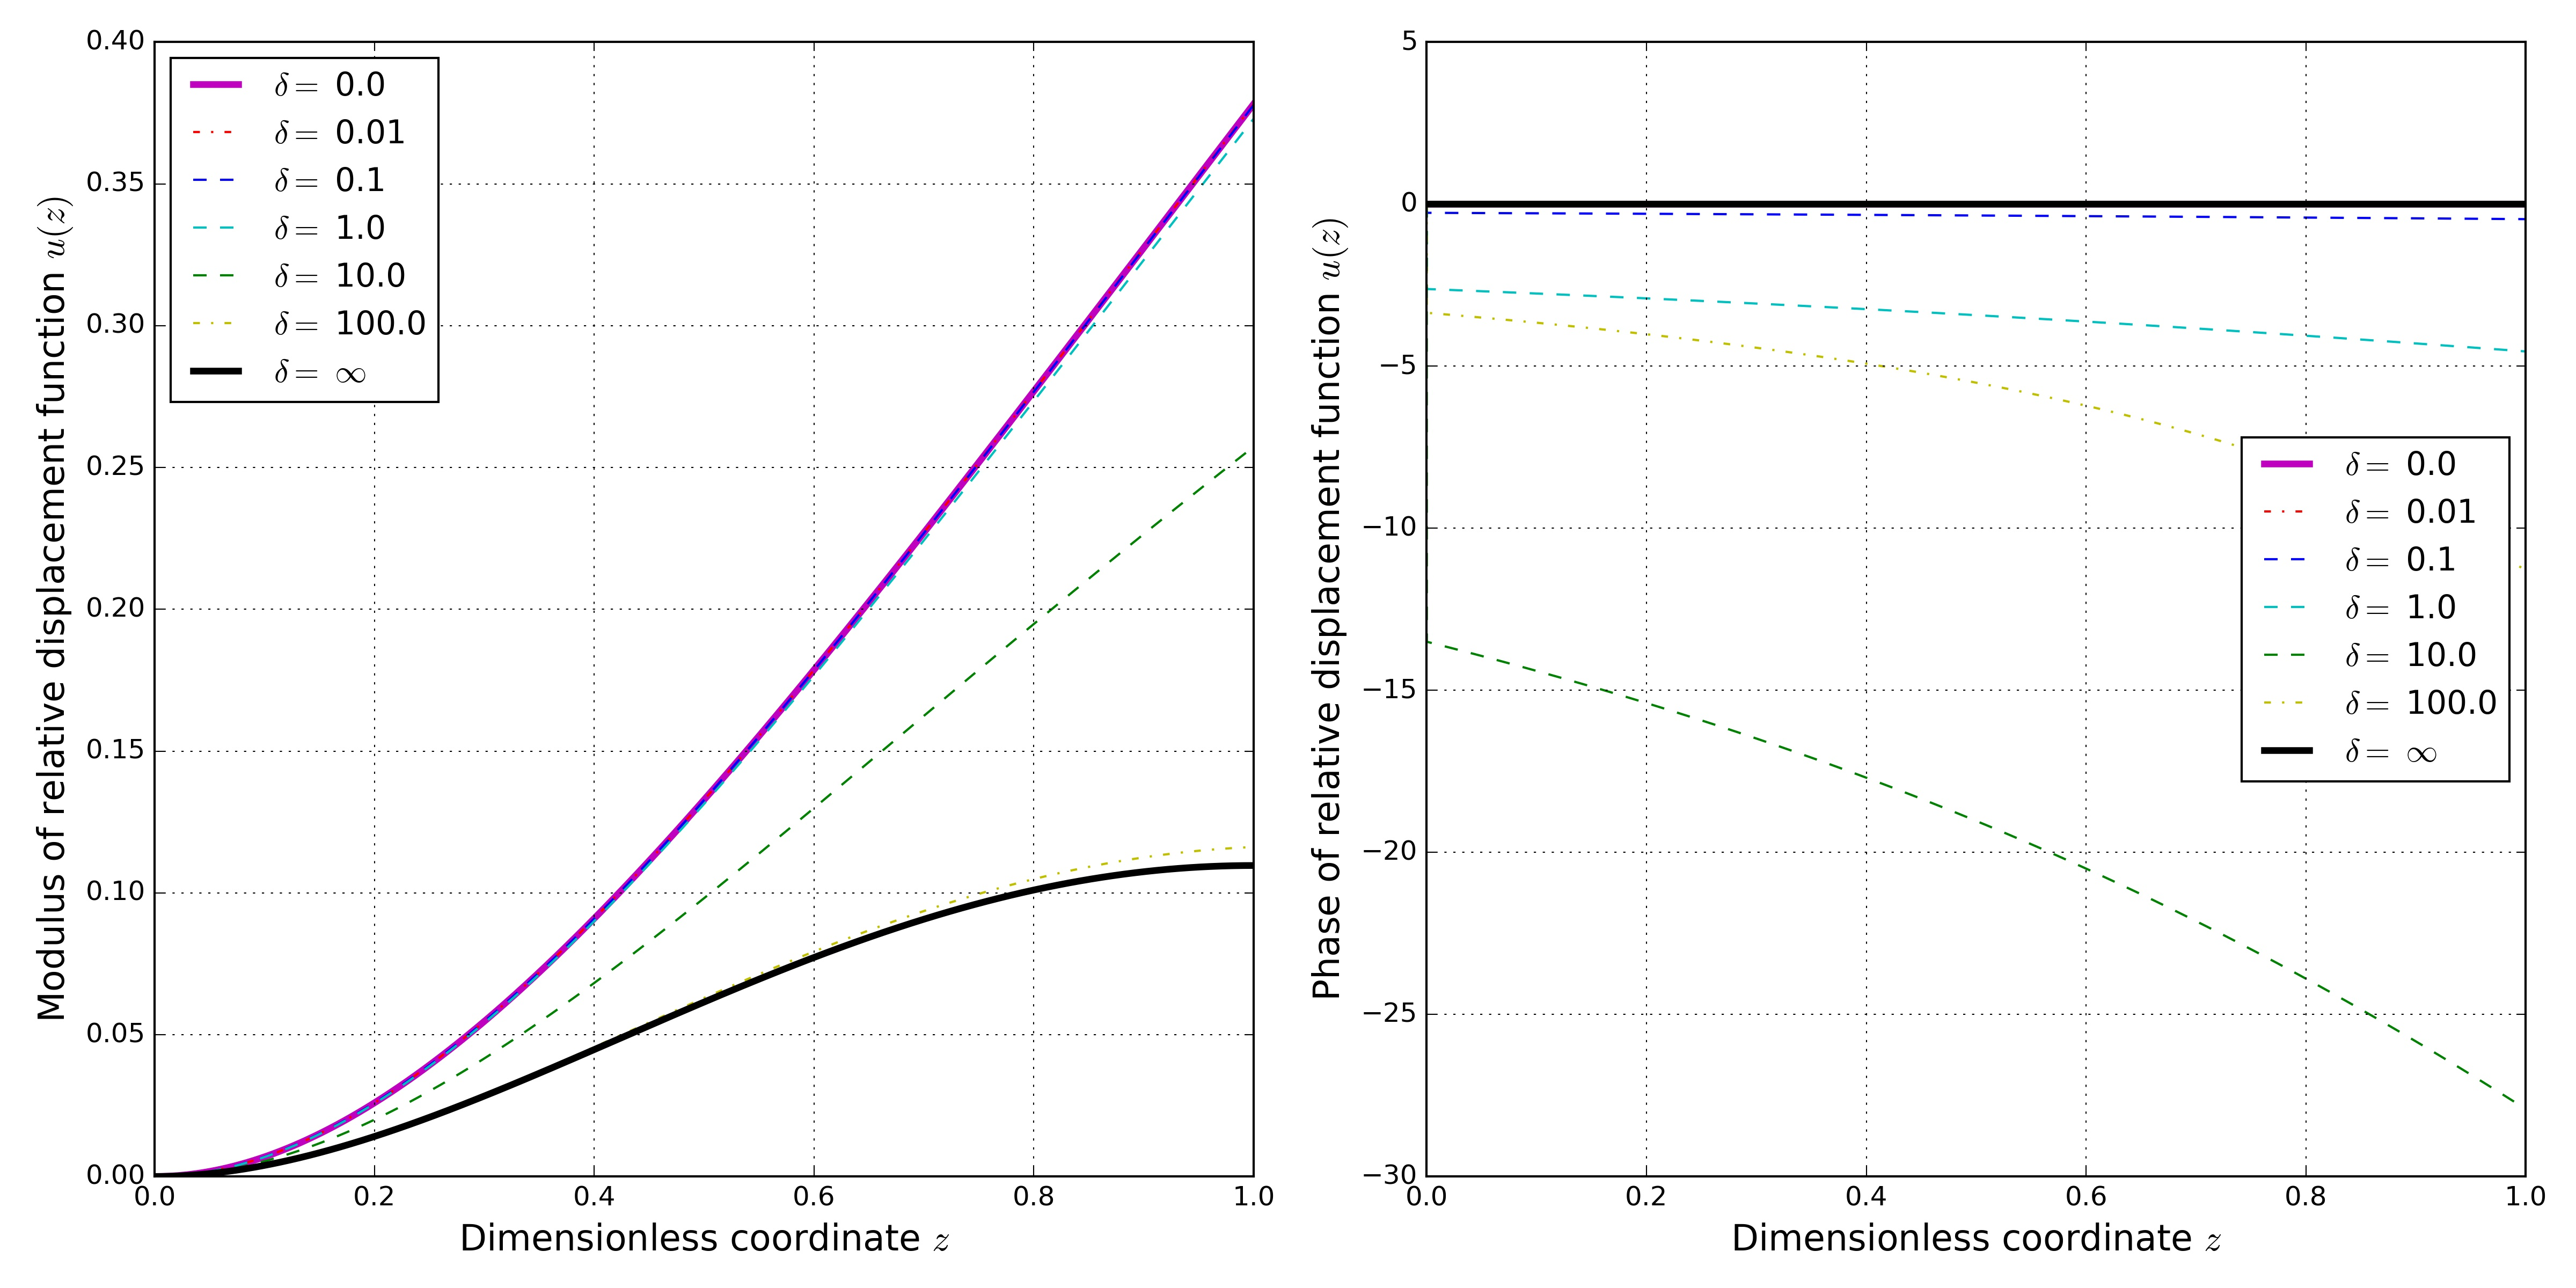
\includegraphics[width=\textwidth]{./img_eig_asy/fig_sol_analytic_disp_fun.jpg}
    \caption{Modulus (left panel) and phase (left panel) of the displacement function $u(z;\delta)$ for different values of $\delta$. Note that for the case of $\delta = 0$ and $\delta = \infty$, the phase is always zero and hence invisible in the figure. The results are calculated at the parameter value of $\beta = 0.064$ and $\sigma = 1.557$.}
    \label{fig:fig_sol_analytic_disp_fun}
\end{figure*}

It is shown in Figure~\ref{fig:fig_sol_analytic_disp_fun} that the parameter $\delta$ changes the function $u(z;\delta)$ through the change of the third boundary condition in the system (\ref{eq:eq_dimensionless_system_all}). When $\delta$ is zero, i.e., no electromechanical coupling is present, the system degenerates to the classical elastic cantilever beam problem, whose solution is a real function. That is to say, the phase of $u(z;\delta)$ is constantly zero across the whole beam (in the range of $0 \leq z \leq 1$).
Analytical expressions for the coefficients in this case are 
\begin{equation}
    \left\{\begin{aligned}
        A_{\varnothing} &= \frac{ 1 + \cos\sqrt{\sigma } \cosh\sqrt{\sigma } - \sin\sqrt{\sigma } \sinh\sqrt{\sigma} }{2 \left[ 1 + \cos\sqrt{\sigma } \cosh\sqrt{\sigma } \right]}, \\
        B_{\varnothing} &= \frac{ \cos\sqrt{\sigma } \sinh\sqrt{\sigma } + \sin\sqrt{\sigma } \cosh\sqrt{\sigma} }{2 \left[ 1 + \cos\sqrt{\sigma } \cosh\sqrt{\sigma } \right]}, \\
        C_{\varnothing} &= \frac{ 1 + \cos\sqrt{\sigma } \cosh\sqrt{\sigma } + \sin\sqrt{\sigma } \sinh\sqrt{\sigma} }{2 \left[ 1 + \cos\sqrt{\sigma } \cosh\sqrt{\sigma } \right]}, \\
        D_{\varnothing} &= \frac{ -\cos\sqrt{\sigma } \sinh\sqrt{\sigma } - \sin\sqrt{\sigma } \cosh\sqrt{\sigma} }{2 \left[ 1 + \cos\sqrt{\sigma } \cosh\sqrt{\sigma } \right]},
    \end{aligned}\right.
    \label{eq:eq_disp_func_coeffs_exps_zero}
\end{equation}
and the resultant dimensionless relative displacement function $u_{\varnothing} (z)$ is represented as
\begin{equation}
    u_{\varnothing} (z) = A_{\varnothing} \cos{\sqrt{\sigma}z} + B_{\varnothing} \sin{\sqrt{\sigma}z} + C_{\varnothing} \cosh{\sqrt{\sigma}z} + D_{\varnothing} \sinh{\sqrt{\sigma}z} - 1.
\end{equation}
When the electromechanical coupling is extremely strong, $\delta$ is extremely large and can be seen as $\infty$ in mathematical sense. In this situation, the solution $u_\infty (z)$ is again real without any phase difference in the $z$ direction. The coefficients can be analytically expressed as 
\begin{equation}
    \left\{\begin{aligned}
        A_\infty &= \frac{ \cos\sqrt{\sigma } \sinh\sqrt{\sigma } }{ \cos\sqrt{\sigma } \sinh\sqrt{\sigma } + \sin\sqrt{\sigma } \cosh\sqrt{\sigma } }, \\
        B_\infty &= \frac{ \sin\sqrt{\sigma } \sinh\sqrt{\sigma } }{ \cos\sqrt{\sigma } \sinh\sqrt{\sigma } + \sin\sqrt{\sigma } \cosh\sqrt{\sigma } }, \\
        C_\infty &= \frac{ \sin\sqrt{\sigma } \cosh\sqrt{\sigma } }{ \cos\sqrt{\sigma } \sinh\sqrt{\sigma } + \sin\sqrt{\sigma } \cosh\sqrt{\sigma } }, \\
        D_\infty &= \frac{ - \sin\sqrt{\sigma } \sinh\sqrt{\sigma } }{ \cos\sqrt{\sigma } \sinh\sqrt{\sigma } + \sin\sqrt{\sigma } \cosh\sqrt{\sigma } },
    \end{aligned}\right.
    \label{eq:eq_disp_func_coeffs_exps_infty}
\end{equation}
and hence the dimensionless relative displacement function $u_{\infty} (z)$ is
\begin{equation}
    u_{\infty} (z) = A_{\infty} \cos{\sqrt{\sigma}z} + B_{\infty} \sin{\sqrt{\sigma}z} + C_{\infty} \cosh{\sqrt{\sigma}z} + D_{\infty} \sinh{\sqrt{\sigma}z} - 1.
\end{equation}
While a finite non-zero electromechanical coupling factor $\delta$ is present, as expected in most applications, modulus and phase of the dimensionless displacement function $u(z;\delta)$ are both changing along the $z$ direction. Nevertheless, it is seen from the right panel of Figure~\ref{fig:fig_sol_analytic_disp_fun} that when the values of $\delta$ is either small or large, the phase change of $u(z;\delta)$ is very small in the $z$ direction. To make it more clear, we plot the modulus and phase of $u(z;\delta)$ at $z=1$ versus different values of $\delta$ in Figure~\ref{fig:fig_sol_analytic_disp_end}. It is clear that with the increase of $\delta$, modulus of $u(1;\delta)$ decreases, while its phase reaches a minimum at some intermediate value of $\delta$ (Here around $\delta = 20$). This also explains the fact expressed in Figure~\ref{fig:fig_sol_analytic_disp_fun} that the modulus of dimensionless relative displacement function $u_\delta (z)$ with $0 < \delta < \infty$ is always between that of $u_\varnothing (z)$ and $u_\infty (z)$.


\begin{figure*}[!htbp]
    \centering
    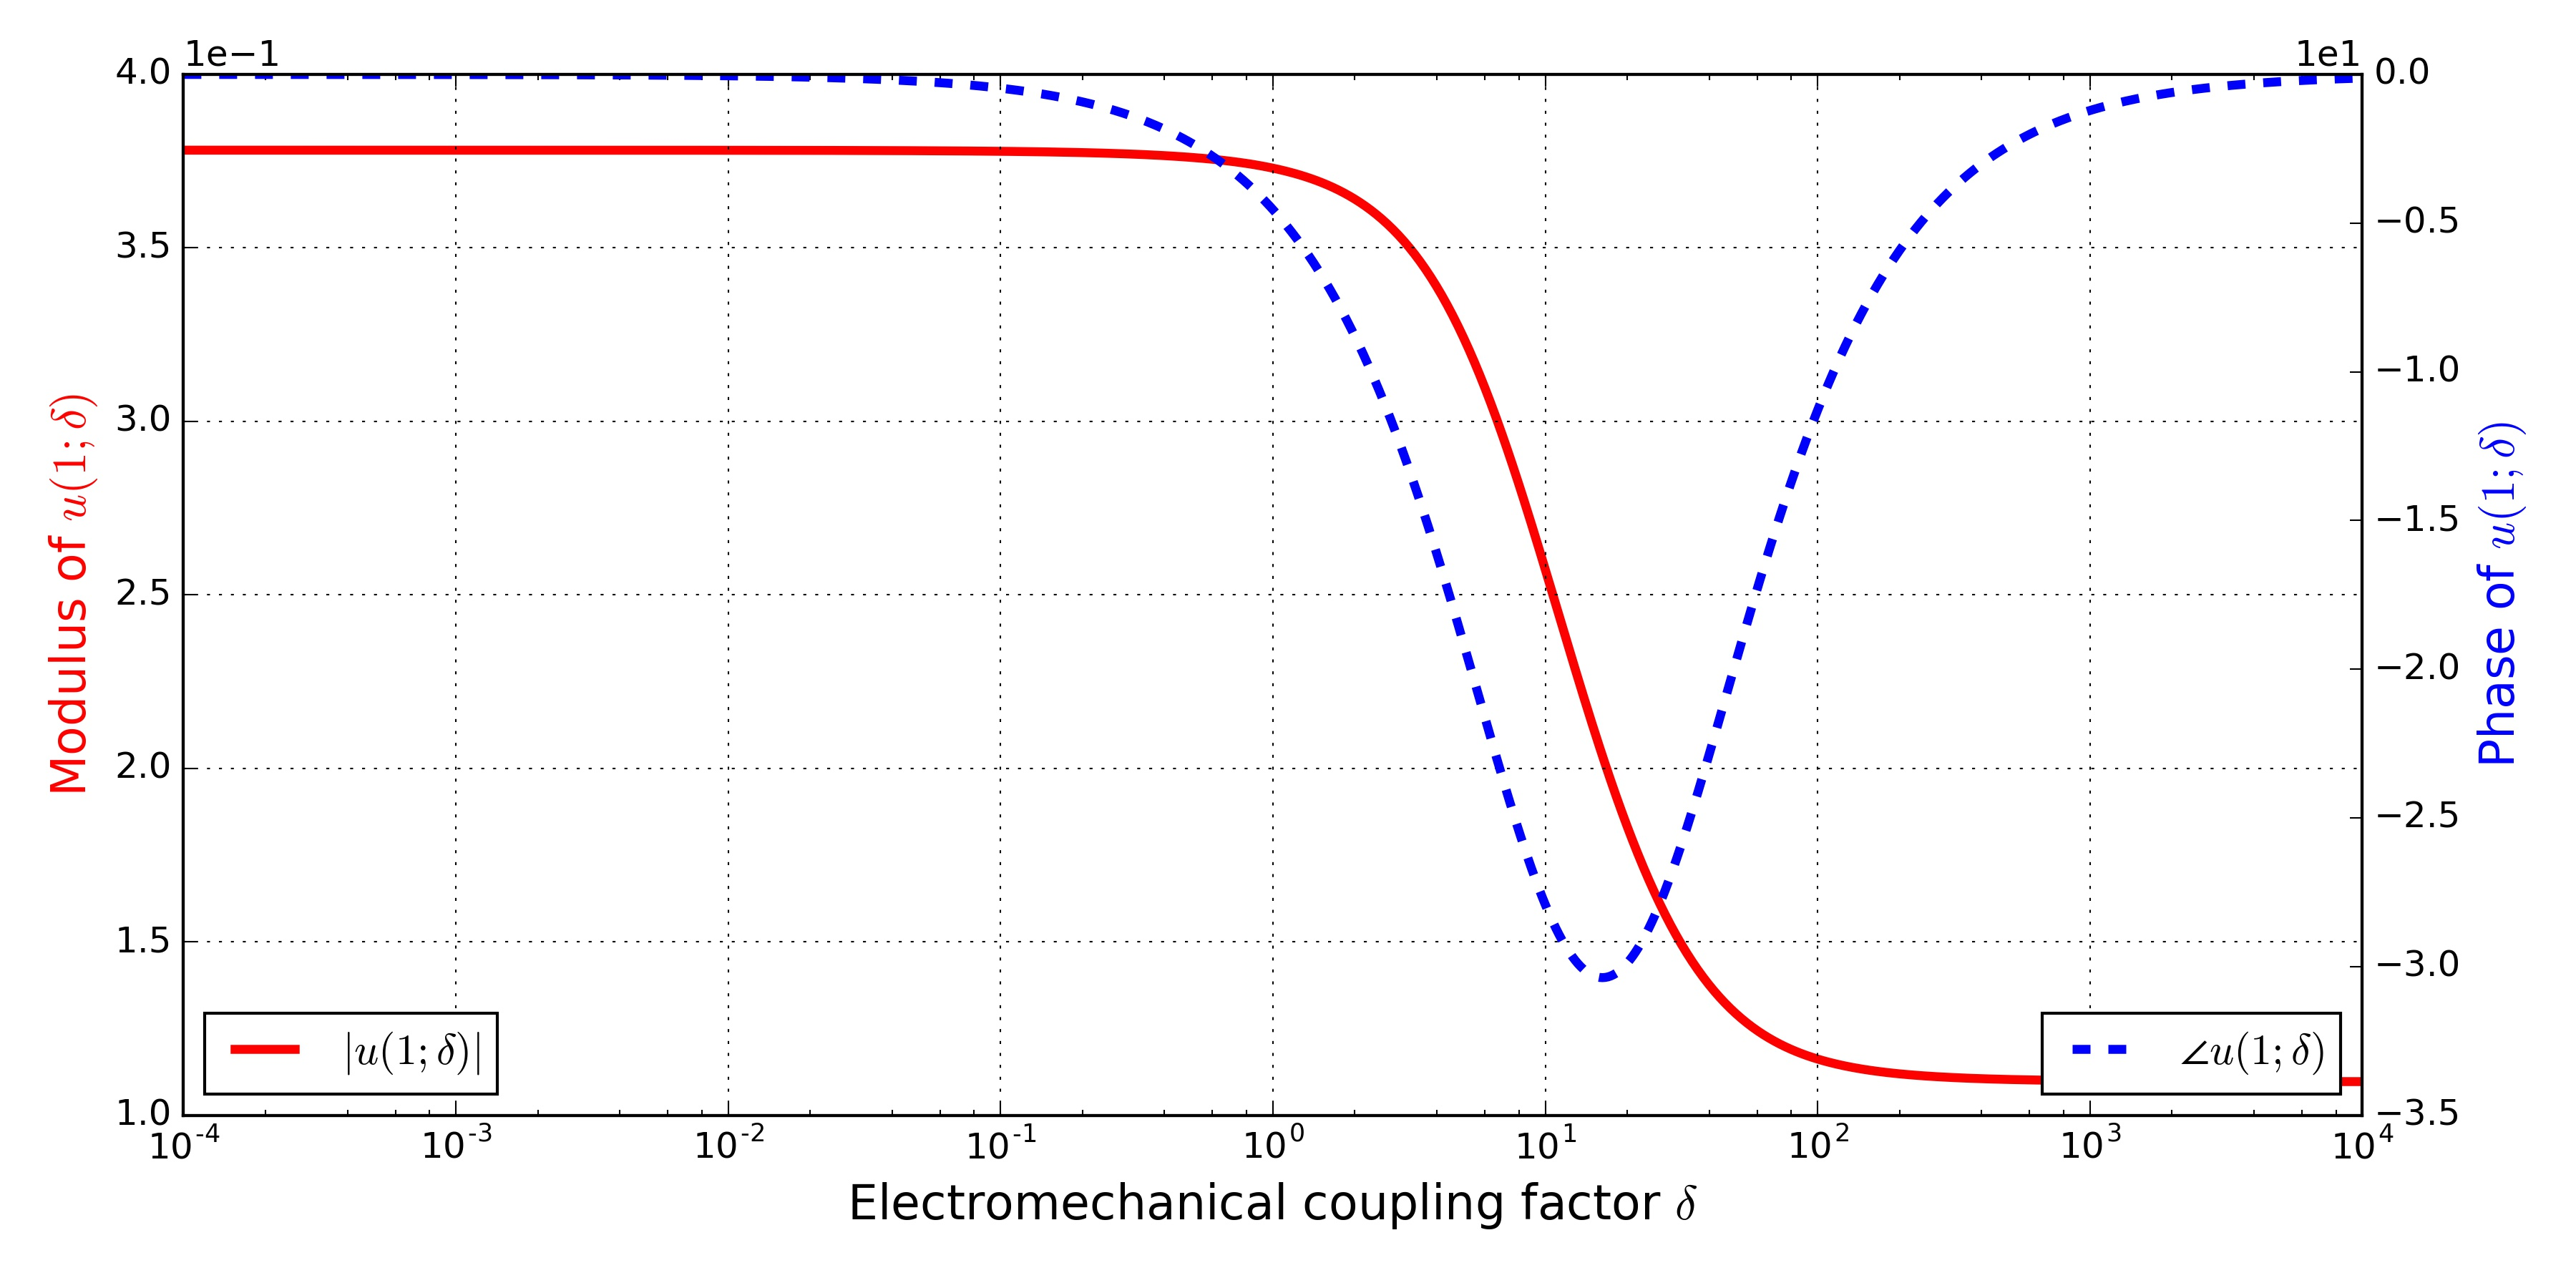
\includegraphics[width=0.8\textwidth]{./img_eig_asy/fig_sol_analytic_disp_end.jpg}
    \caption{Modulus and phase of the displacement function $u(z;\delta)$ at the position $z=1$ versus electromechanical coupling factor $\delta$. The results are calculated at the parameter value of $\beta = 0.064$ and $\sigma = 1.557$.}
    \label{fig:fig_sol_analytic_disp_end}
\end{figure*}



As for the output voltage $V_p(t)$, output current $I_p(t)$, and output power $P_p(t)$ of the PVEH, the corresponding complex amplitudes $\tilde{V}_p$, $\tilde{I}_p$, and $\tilde{P}_p$ can be formulated as
\begin{equation}
    \left\{\begin{aligned}
        \tilde{V}_p &= -\frac{j \sigma \beta}{j \sigma \beta + 1} \frac{\eta_b}{l_p} \frac{e_p}{C_p} u^\prime(1) = -\frac{j \sigma \beta}{j \sigma \beta + 1} \frac{\eta_b}{l_p} \frac{e_p}{C_p} \chi_p, \\
        \tilde{I}_p &=  \tilde{V}_p / R_l = - \frac{ j \sigma \beta } {j \sigma \beta + 1} \left( \frac{\eta_b}{l_p} \right) \left( \frac{e_p}{C_p R_l} \right) \chi_p , \\
        \tilde{P}_p &=  \tilde{V}_p^2 / R_l = \left(\frac{\eta_b}{l_p}\right)^2 \left(\frac{e_p}{C_p}\right) \left( \frac{e_p}{C_p R_l} \right) \left( \frac{ j \sigma \beta}{ j \sigma \beta + 1 } \right)^2 \chi_p^2,
    \end{aligned}\right.
    \label{eq:eq_peh_perfs_compact_form}
\end{equation}
in which we have used the notations of output index $\chi_p$ 
\begin{equation}
    \chi_p = u_1^\prime(1) = \frac{ \sqrt{\sigma} \left( \sinh\sqrt{\sigma} - \sin\sqrt{\sigma} \right) }{ 1 + \cos\sqrt{\sigma } \cosh\sqrt{\sigma } + \frac{j \beta \sqrt{\sigma}}{ 1+ j \beta \sigma } \delta \left( \cos\sqrt{\sigma } \sinh\sqrt{\sigma } + \sin\sqrt{\sigma } \cosh\sqrt{\sigma } \right) }.
    \label{eq:eq_peh_perfs_compact_form_end_ders}
\end{equation}
Clearly, The three output measures $\tilde{V}_p$, $\tilde{I}_p$, and $\tilde{P}_p$ are heavily dependent on another dimensionless parameter $r_d = \eta_b/l_p$, which is the dimensionless base excitation amplitude. Formally, both $\tilde{V}_p$ and $\tilde{I}_p$ depend linearly upon $r_d$, while $\tilde{P}_p$ shows a quadratic dependence on $r_d$. The only dependence upon $\delta$ is introduced in $\chi_p$. However, it should be noted that the definition of parameter $\delta$ relies on $e_p$, $l_p$, $C_p$, and $B_p$, while the three measures $\tilde{V}_p$, $\tilde{I}_p$, and $\tilde{P}_p$ are dimensional values and depend on $e_p$, $\sigma_b$, and $R_l$. As a result, the change of parameter $\delta$ results in the change of reference voltage $e_p / C_p$, reference current $e_p / (C_p R_l)$, and reference power $(e_p / C_p)[e_p / (C_p R_l)]$, and therefore the corresponding values of $\tilde{V}_p$, $\tilde{I}_p$, and $\tilde{P}_p$. Hence, we may establish a bijective relation between $\delta$ and $e_p$, and relate the change of $\delta$ to that of $e_p$. In this way, we calculate the three output measures $\tilde{V}_p$, $\tilde{I}_p$, and $\tilde{P}_p$ at different values of $\delta$ and plot their moduli in Figure~\ref{fig:fig_sol_analytic_perf_fun}.

\begin{figure*}[!htbp]
    \centering
    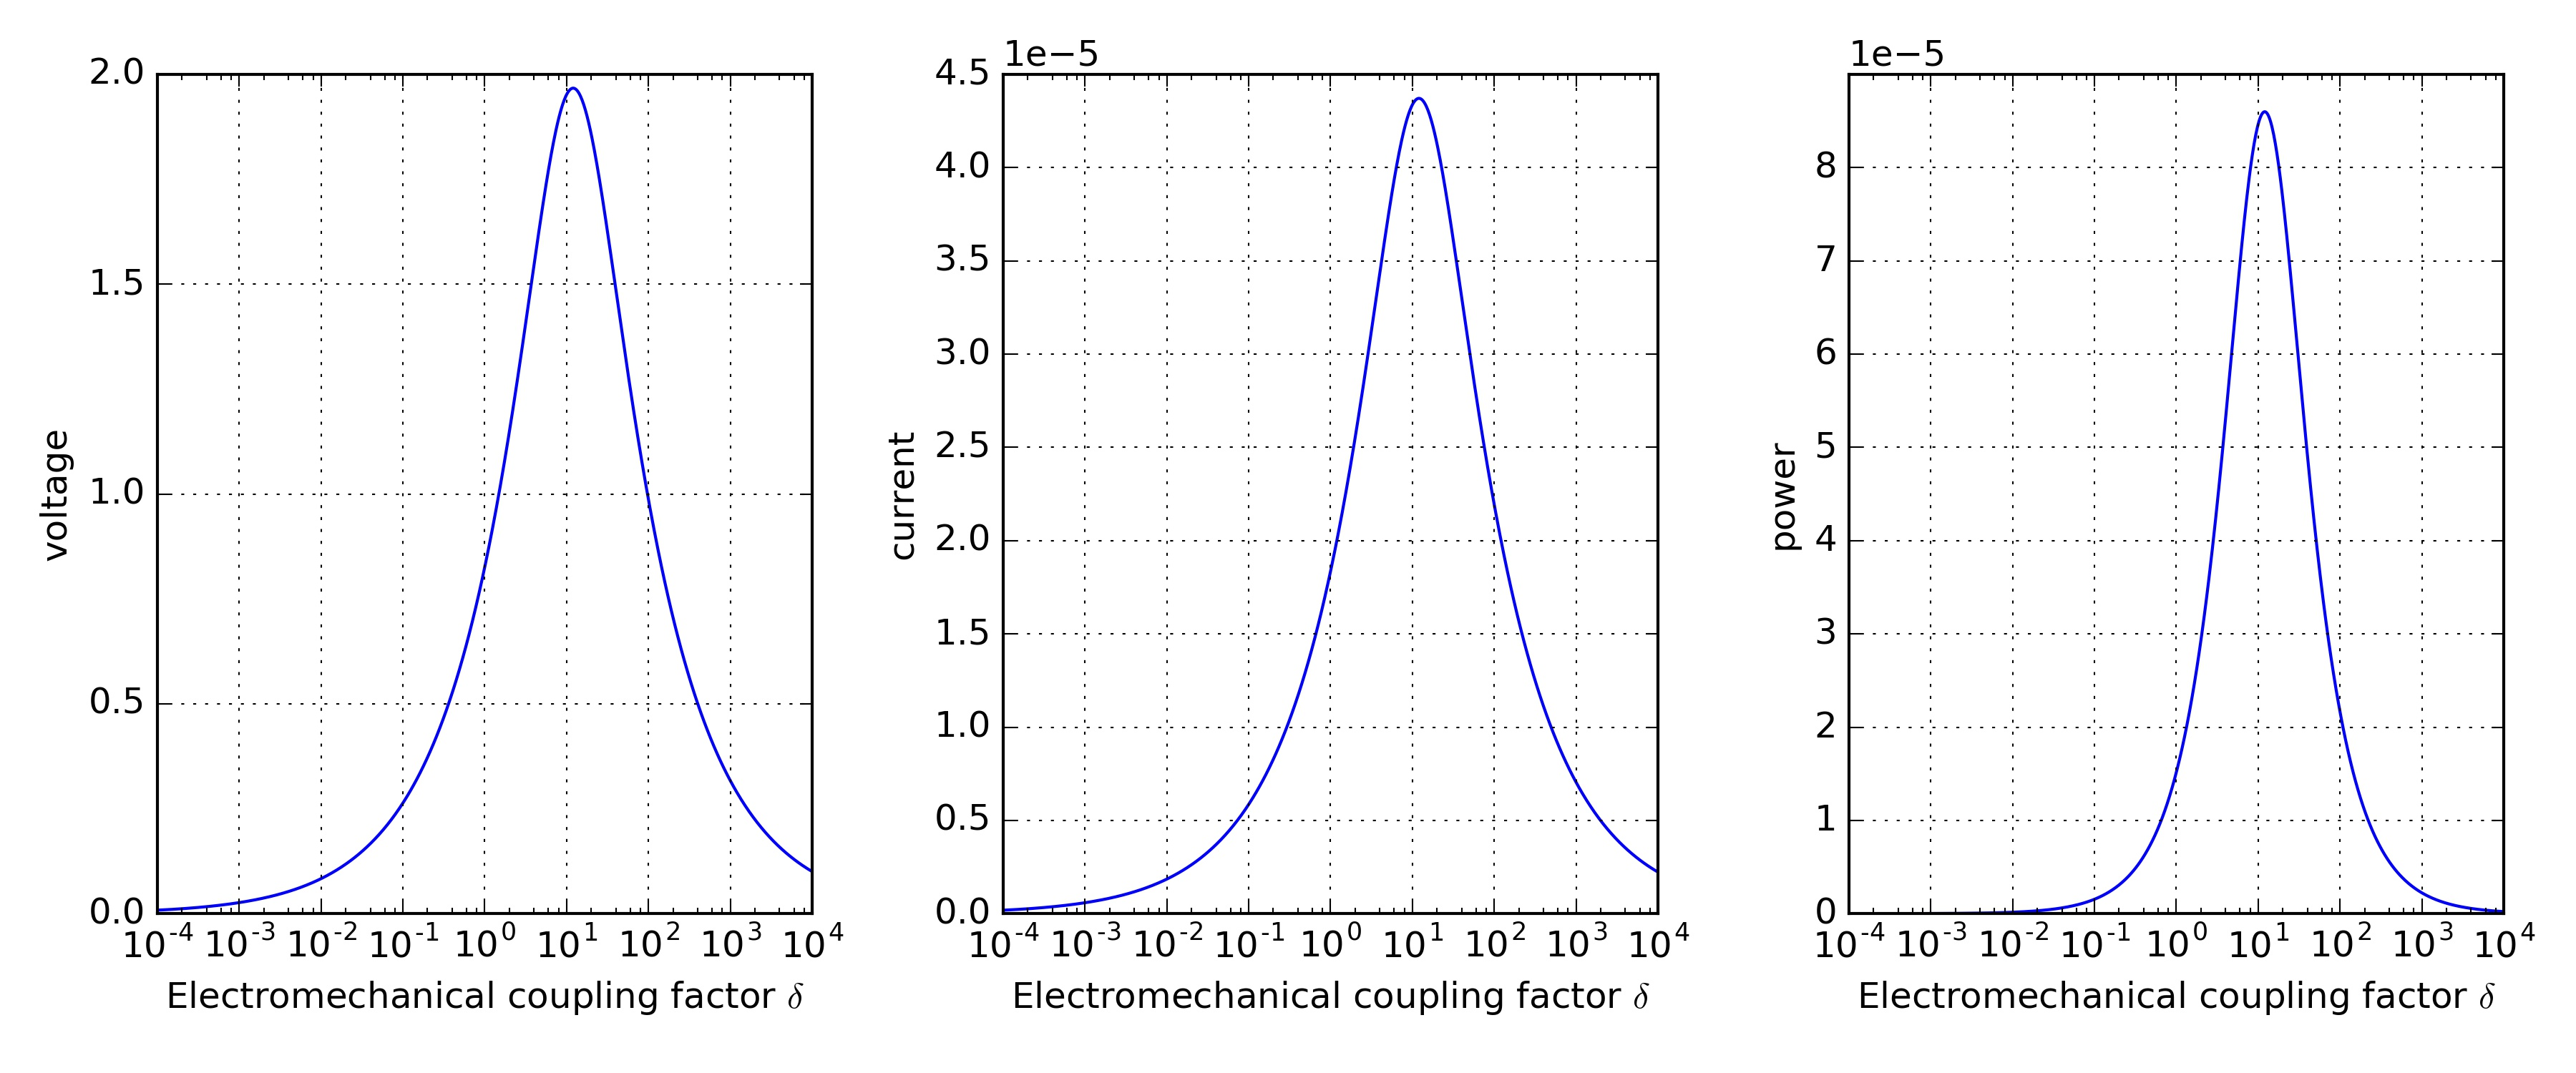
\includegraphics[width=\textwidth]{./img_eig_asy/fig_sol_analytic_perf_fun}
    \caption{Output voltage amplitude $\tilde{V}_p$, output current current $\tilde{I}_p$, and output power amplitude $\tilde{P}_p$ for the PVEH as a function of electromechanical coupling factor $\delta$ and equivalently $e_p$. The results are calculated at the parameter value of $\beta = 0.064$ and $\sigma = 1.557$.}
    \label{fig:fig_sol_analytic_perf_fun}
\end{figure*}


It is seen from Figure~\ref{fig:fig_sol_analytic_perf_fun} that all the three output measures $\tilde{V}_p$, $\tilde{I}_p$, and $\tilde{P}_p$ show a maximum peak with the increase of $\delta$ at the approximate value of $\delta = 10$. When $\delta$ is small, or equivalently, $e_p$ is small, amplitudes of the three output measures $\tilde{V}_p$, $\tilde{I}_p$, and $\tilde{P}_p$ increase with the increase of $\delta$. Then after the critical value of $\delta$, a further increase of $\delta$ causes the decrease of these three output measures. Thus we come to a small conclusion that to obtain an optimal output performance, the electromechanical coupling factor $\delta$ should be set to an appropriate value. However, a direct calculation using the parameters introduced in the literature \cite{erturk2008distributed,erturk2009experimentally} shows that the parameter $\delta$ is rather small for a typical PVEH. For example, for a piezoelectric voltage constant $e_{31} = --12.54\ C / m^2$, the value of $e_p$ is $-8.778 \times 10^{-5}\ C$, and the final value of $\delta$ is $0.111$. According to the properties of commonly used piezoelectric materials, the parameter $e_{31}$ is always in the range of several or several tens $C / m^2$ \cite{erturk2011piezoelectric}. That is to say, the final value of $\delta$ is always in the order of $10^{-2}$ to $10^{-1}$, which is a rather small value according to the diagram. Hence we could present an asymptotic analysis of the performance of the PVEH. This is the subject of the following section.


\section{Asymptotic analysis of the model}

According to the above analysis, for small values of the parameter $\delta$, our solution to the derived model can be expanded in the following way:
\begin{equation}
    \left\{\begin{aligned}
        A_\delta &= A_0 + \delta A_1 + \delta^2 A_2 + \cdots, \\
        B_\delta &= B_0 + \delta B_1 + \delta^2 B_2 + \cdots, \\
        C_\delta &= C_0 + \delta C_1 + \delta^2 C_2 + \cdots, \\
        D_\delta &= D_0 + \delta D_1 + \delta^2 D_2 + \cdots. 
    \end{aligned}\right.
\end{equation}
As a result, we obtain the following successive expansion problem:

\noindent
$O(\delta^0)$:
\begin{equation}
    \left\{\begin{aligned}
        A_0 + C_0 &= 1, \\
        B_0 + D_0 &= 0, \\
        - A_0 \cos{\sqrt{\sigma}} - B_0 \sin{\sqrt{\sigma}} + C_0 \cosh{\sqrt{\sigma}} + D_0 \sinh{\sqrt{\sigma}} &= 0, \\
        A_0 \sin{\sqrt{\sigma}} - B_0 \cos{\sqrt{\sigma}} + C_0 \sinh{\sqrt{\sigma}} + D_0 \cosh{\sqrt{\sigma}} &= 0.
    \end{aligned}\right.
\end{equation}
The solution is
\begin{equation}
    \left\{\begin{aligned}
        A_0 &= \frac{1 + \cos\sqrt{\sigma} \cosh\sqrt{\sigma} - \sin\sqrt{\sigma} \sinh\sqrt{\sigma} }{2 + 2 \cos\sqrt{\sigma} \cosh\sqrt{\sigma} }, \\
        B_0 &= \frac{\cosh\sqrt{\sigma} \sin\sqrt{\sigma} + \cos\sqrt{\sigma} \sinh\sqrt{\sigma} }{2 + 2 \cos\sqrt{\sigma} \cosh\sqrt{\sigma} }, \\
        C_0 &= \frac{1 + \cos\sqrt{\sigma} \cosh\sqrt{\sigma} + \sin\sqrt{\sigma} \sinh\sqrt{\sigma} }{2 + 2 \cos\sqrt{\sigma} \cosh\sqrt{\sigma} }, \\
        D_0 &= -\frac{\cosh\sqrt{\sigma} \sin\sqrt{\sigma} + \cos\sqrt{\sigma} \sinh\sqrt{\sigma} }{2 + 2 \cos\sqrt{\sigma} \cosh\sqrt{\sigma} }.
    \end{aligned}\right.
\end{equation}
Hence we have
\begin{equation}
    - A_0 \sin{\sqrt{\sigma}} + B_0 \cos{\sqrt{\sigma}} + C_0 \sinh{\sqrt{\sigma}} + D_0 \cosh{\sqrt{\sigma}} = \frac{\sinh\sqrt{\sigma }-\sin\sqrt{\sigma }}{\cos\sqrt{\sigma } \cosh\sqrt{\sigma }+1}
\end{equation}

\noindent
$O(\delta^1)$:
\begin{equation}
    \left\{\begin{aligned}
        A_1 + C_1 &= 0, \\
        B_1 + D_1 &= 0, \\
        \left( - A_1 \cos{\sqrt{\sigma}} - B_1 \sin{\sqrt{\sigma}} + C_1 \cosh{\sqrt{\sigma}} + D_1 \sinh{\sqrt{\sigma}} \right) &+ \\
        \frac{j \beta \sqrt{\sigma}}{ j\sigma \beta + 1 } \left( - A_0 \sin{\sqrt{\sigma}} + B_0 \cos{\sqrt{\sigma}} + C_0 \sinh{\sqrt{\sigma}} + D_0 \cosh{\sqrt{\sigma}} \right) &= 0, \\
        A_1 \sin{\sqrt{\sigma}} - B_1 \cos{\sqrt{\sigma}} + C_1 \sinh{\sqrt{\sigma}} + D_1 \cosh{\sqrt{\sigma}} &= 0.
    \end{aligned}\right.
\end{equation}
The solution is
\begin{equation}
    \left\{\begin{aligned}
        A_1 &= \frac{j \beta  \sqrt{\sigma }}{1+j \beta  \sigma } \left( \frac{\sinh\sqrt{\sigma }-\sin\sqrt{\sigma }}{\cos\sqrt{\sigma } \cosh\sqrt{\sigma }+1} \right) \left(\frac{\cos\sqrt{\sigma }+\cosh\sqrt{\sigma }}{2 \cos\sqrt{\sigma }\cosh\sqrt{\sigma }+2} \right) \\
        B_1 &= \frac{j \beta  \sqrt{\sigma }}{1+j \beta  \sigma } \left( \frac{\sinh\sqrt{\sigma }-\sin\sqrt{\sigma }}{\cos\sqrt{\sigma } \cosh\sqrt{\sigma }+1} \right) \left( \frac{-\sinh\sqrt{\sigma }+\sin\sqrt{\sigma }}{2 \cos\sqrt{\sigma }\cosh\sqrt{\sigma }+2} \right)\\
        C_1 &= \frac{j \beta  \sqrt{\sigma }}{1+j \beta  \sigma } \left( \frac{\sinh\sqrt{\sigma }-\sin\sqrt{\sigma }}{\cos\sqrt{\sigma } \cosh\sqrt{\sigma }+1} \right) \left( -\frac{\cos\sqrt{\sigma }+\cosh\sqrt{\sigma }}{2 \cos\sqrt{\sigma } \cosh\sqrt{\sigma }+2} \right)\\
        D_1 &= \frac{j \beta  \sqrt{\sigma }}{1+j \beta  \sigma } \left( \frac{\sinh\sqrt{\sigma }-\sin\sqrt{\sigma }}{\cos\sqrt{\sigma } \cosh\sqrt{\sigma }+1} \right) \left( \frac{-\sin\sqrt{\sigma }+\sinh\sqrt{\sigma }}{2 \cos\sqrt{\sigma }\cosh\sqrt{\sigma }+2} \right)
    \end{aligned}\right.
\end{equation}
Then we have
\begin{equation}
    \begin{aligned}
        - A_1 \sin{\sqrt{\sigma}} + B_1 \cos{\sqrt{\sigma}} + C_1 \sinh{\sqrt{\sigma}} + D_1 \cosh{\sqrt{\sigma}} \\
        = \frac{j \beta  \sqrt{\sigma }}{1+j \beta  \sigma } \left(\frac{\sin\sqrt{\sigma } -\sinh\sqrt{\sigma }}{\cos\sqrt{\sigma } \cosh\sqrt{\sigma }+1} \right)  \left( \frac{\cos\sqrt{\sigma } \sinh\sqrt{\sigma }+\sin\sqrt{\sigma } \cosh\sqrt{\sigma }}{\cos\sqrt{\sigma } \cosh\sqrt{\sigma }+1} \right)
    \end{aligned}
\end{equation}

\noindent
$O(\delta^2)$:
\begin{equation}
    \left\{\begin{aligned}
        A_2 + C_2 &= 0, \\
        B_2 + D_2 &= 0, \\
        \left( - A_2 \cos{\sqrt{\sigma}} - B_2 \sin{\sqrt{\sigma}} + C_2 \cosh{\sqrt{\sigma}} + D_2 \sinh{\sqrt{\sigma}} \right) &+ \\
        \frac{j \beta \sqrt{\sigma}}{ j\sigma \beta + 1 } \left( - A_1 \sin{\sqrt{\sigma}} + B_1 \cos{\sqrt{\sigma}} + C_1 \sinh{\sqrt{\sigma}} + D_1 \cosh{\sqrt{\sigma}} \right) &= 0, \\
        A_2 \sin{\sqrt{\sigma}} - B_2 \cos{\sqrt{\sigma}} + C_2 \sinh{\sqrt{\sigma}} + D_2 \cosh{\sqrt{\sigma}} &= 0.
    \end{aligned}\right.
\end{equation}
The solution is
\scriptsize
\begin{equation}
    \left\{\begin{aligned}
        A_2 &= \left( \frac{j \beta \sqrt{\sigma }}{1+j \beta \sigma } \right)^2 \left(\frac{ \sinh\sqrt{\sigma } - \sin\sqrt{\sigma }}{\cos\sqrt{\sigma } \cosh\sqrt{\sigma }+1} \right) \left( \frac{\cos\sqrt{\sigma } \sinh\sqrt{\sigma }+\sin\sqrt{\sigma } \cosh\sqrt{\sigma }}{\cos\sqrt{\sigma } \cosh\sqrt{\sigma }+1} \right) \left(\frac{\cos\sqrt{\sigma }+\cosh\sqrt{\sigma }}{2 \cos\sqrt{\sigma }\cosh\sqrt{\sigma }+2} \right) \\
        B_2 &= \left( \frac{j \beta \sqrt{\sigma }}{1+j \beta \sigma } \right)^2 \left(\frac{\sinh\sqrt{\sigma } - \sin\sqrt{\sigma }}{\cos\sqrt{\sigma } \cosh\sqrt{\sigma }+1} \right) \left( \frac{\cos\sqrt{\sigma } \sinh\sqrt{\sigma }+\sin\sqrt{\sigma } \cosh\sqrt{\sigma }}{\cos\sqrt{\sigma } \cosh\sqrt{\sigma }+1} \right) \left( \frac{-\sinh\sqrt{\sigma }+\sin\sqrt{\sigma }}{2 \cos\sqrt{\sigma }\cosh\sqrt{\sigma }+2} \right)\\
        C_2 &= \left( \frac{j \beta \sqrt{\sigma }}{1+j \beta \sigma } \right)^2 \left(\frac{\sinh\sqrt{\sigma } - \sin\sqrt{\sigma }}{\cos\sqrt{\sigma } \cosh\sqrt{\sigma }+1} \right) \left( \frac{\cos\sqrt{\sigma } \sinh\sqrt{\sigma }+\sin\sqrt{\sigma } \cosh\sqrt{\sigma }}{\cos\sqrt{\sigma } \cosh\sqrt{\sigma }+1} \right) \left( -\frac{\cos\sqrt{\sigma }+\cosh\sqrt{\sigma }}{2 \cos\sqrt{\sigma } \cosh\sqrt{\sigma }+2} \right)\\
        D_2 &= \left( \frac{j \beta \sqrt{\sigma }}{1+j \beta \sigma } \right)^2 \left(\frac{\sinh\sqrt{\sigma } - \sin\sqrt{\sigma }}{\cos\sqrt{\sigma } \cosh\sqrt{\sigma }+1} \right) \left( \frac{\cos\sqrt{\sigma } \sinh\sqrt{\sigma }+\sin\sqrt{\sigma } \cosh\sqrt{\sigma }}{\cos\sqrt{\sigma } \cosh\sqrt{\sigma }+1} \right) \left( \frac{-\sin\sqrt{\sigma }+\sinh\sqrt{\sigma }}{2 \cos\sqrt{\sigma }\cosh\sqrt{\sigma }+2} \right)
    \end{aligned}\right.
\end{equation}
\normalsize

Indeed, we can continue to obtain the coefficients for higher order expansions, as shown in the appendix. Nevertheless, it suffices here to consider only the expansions up to the second order, which are represented by $u^{(0)} (z)$, $u^{(1)} (z)$, and $u^{(2)} (z)$, respectively:
\begin{equation}
    \left\{\begin{aligned}
        u^{(0)} (z) &= u_0 (z), \\
        u^{(1)} (z) &= u_0 (z) + \delta u_1(z), \\
        u^{(2)} (z) &= u_0 (z) + \delta u_1(z) + \delta^2 u_2 (z),
    \end{aligned}\right.
\end{equation}
where the terms $u_0 (z)$, $u_1(z)$, and $u_2 (z)$ are defined as
\begin{equation}
    \left\{\begin{aligned}
        u_0 (z) &= A_0 \cos{\sqrt{\sigma}z} + B_0 \sin{\sqrt{\sigma}z} + C_0 \cosh{\sqrt{\sigma}z} + D_0 \sinh{\sqrt{\sigma}z} - 1, \\
        u_1 (z) &= A_1 \cos{\sqrt{\sigma}z} + B_1 \sin{\sqrt{\sigma}z} + C_1 \cosh{\sqrt{\sigma}z} + D_1 \sinh{\sqrt{\sigma}z}, \\
        u_2 (z) &= A_2 \cos{\sqrt{\sigma}z} + B_2 \sin{\sqrt{\sigma}z} + C_2 \cosh{\sqrt{\sigma}z} + D_2 \sinh{\sqrt{\sigma}z}.
    \end{aligned}\right.
\end{equation}

For different values of $\delta$ and $\sigma$ (Here in this simulation, the value of $\sigma$ is changed through the variance of base excitation frequency $f_b$), the asymptotic approximations of the dimensionless relative beam displacement function $u(z;\delta)$ up to the second order $u^{(0)}(z)$, $u^{(1)}(z)$, and $u^{(2)}(z)$ are calculated and compared to the solution $u(z;\delta)$ itself. The results are shown in Figure~\ref{fig:fig_sol_analytic_disp_cmp_fr_all}. 

\begin{figure*}[!htbp]
    \centering
    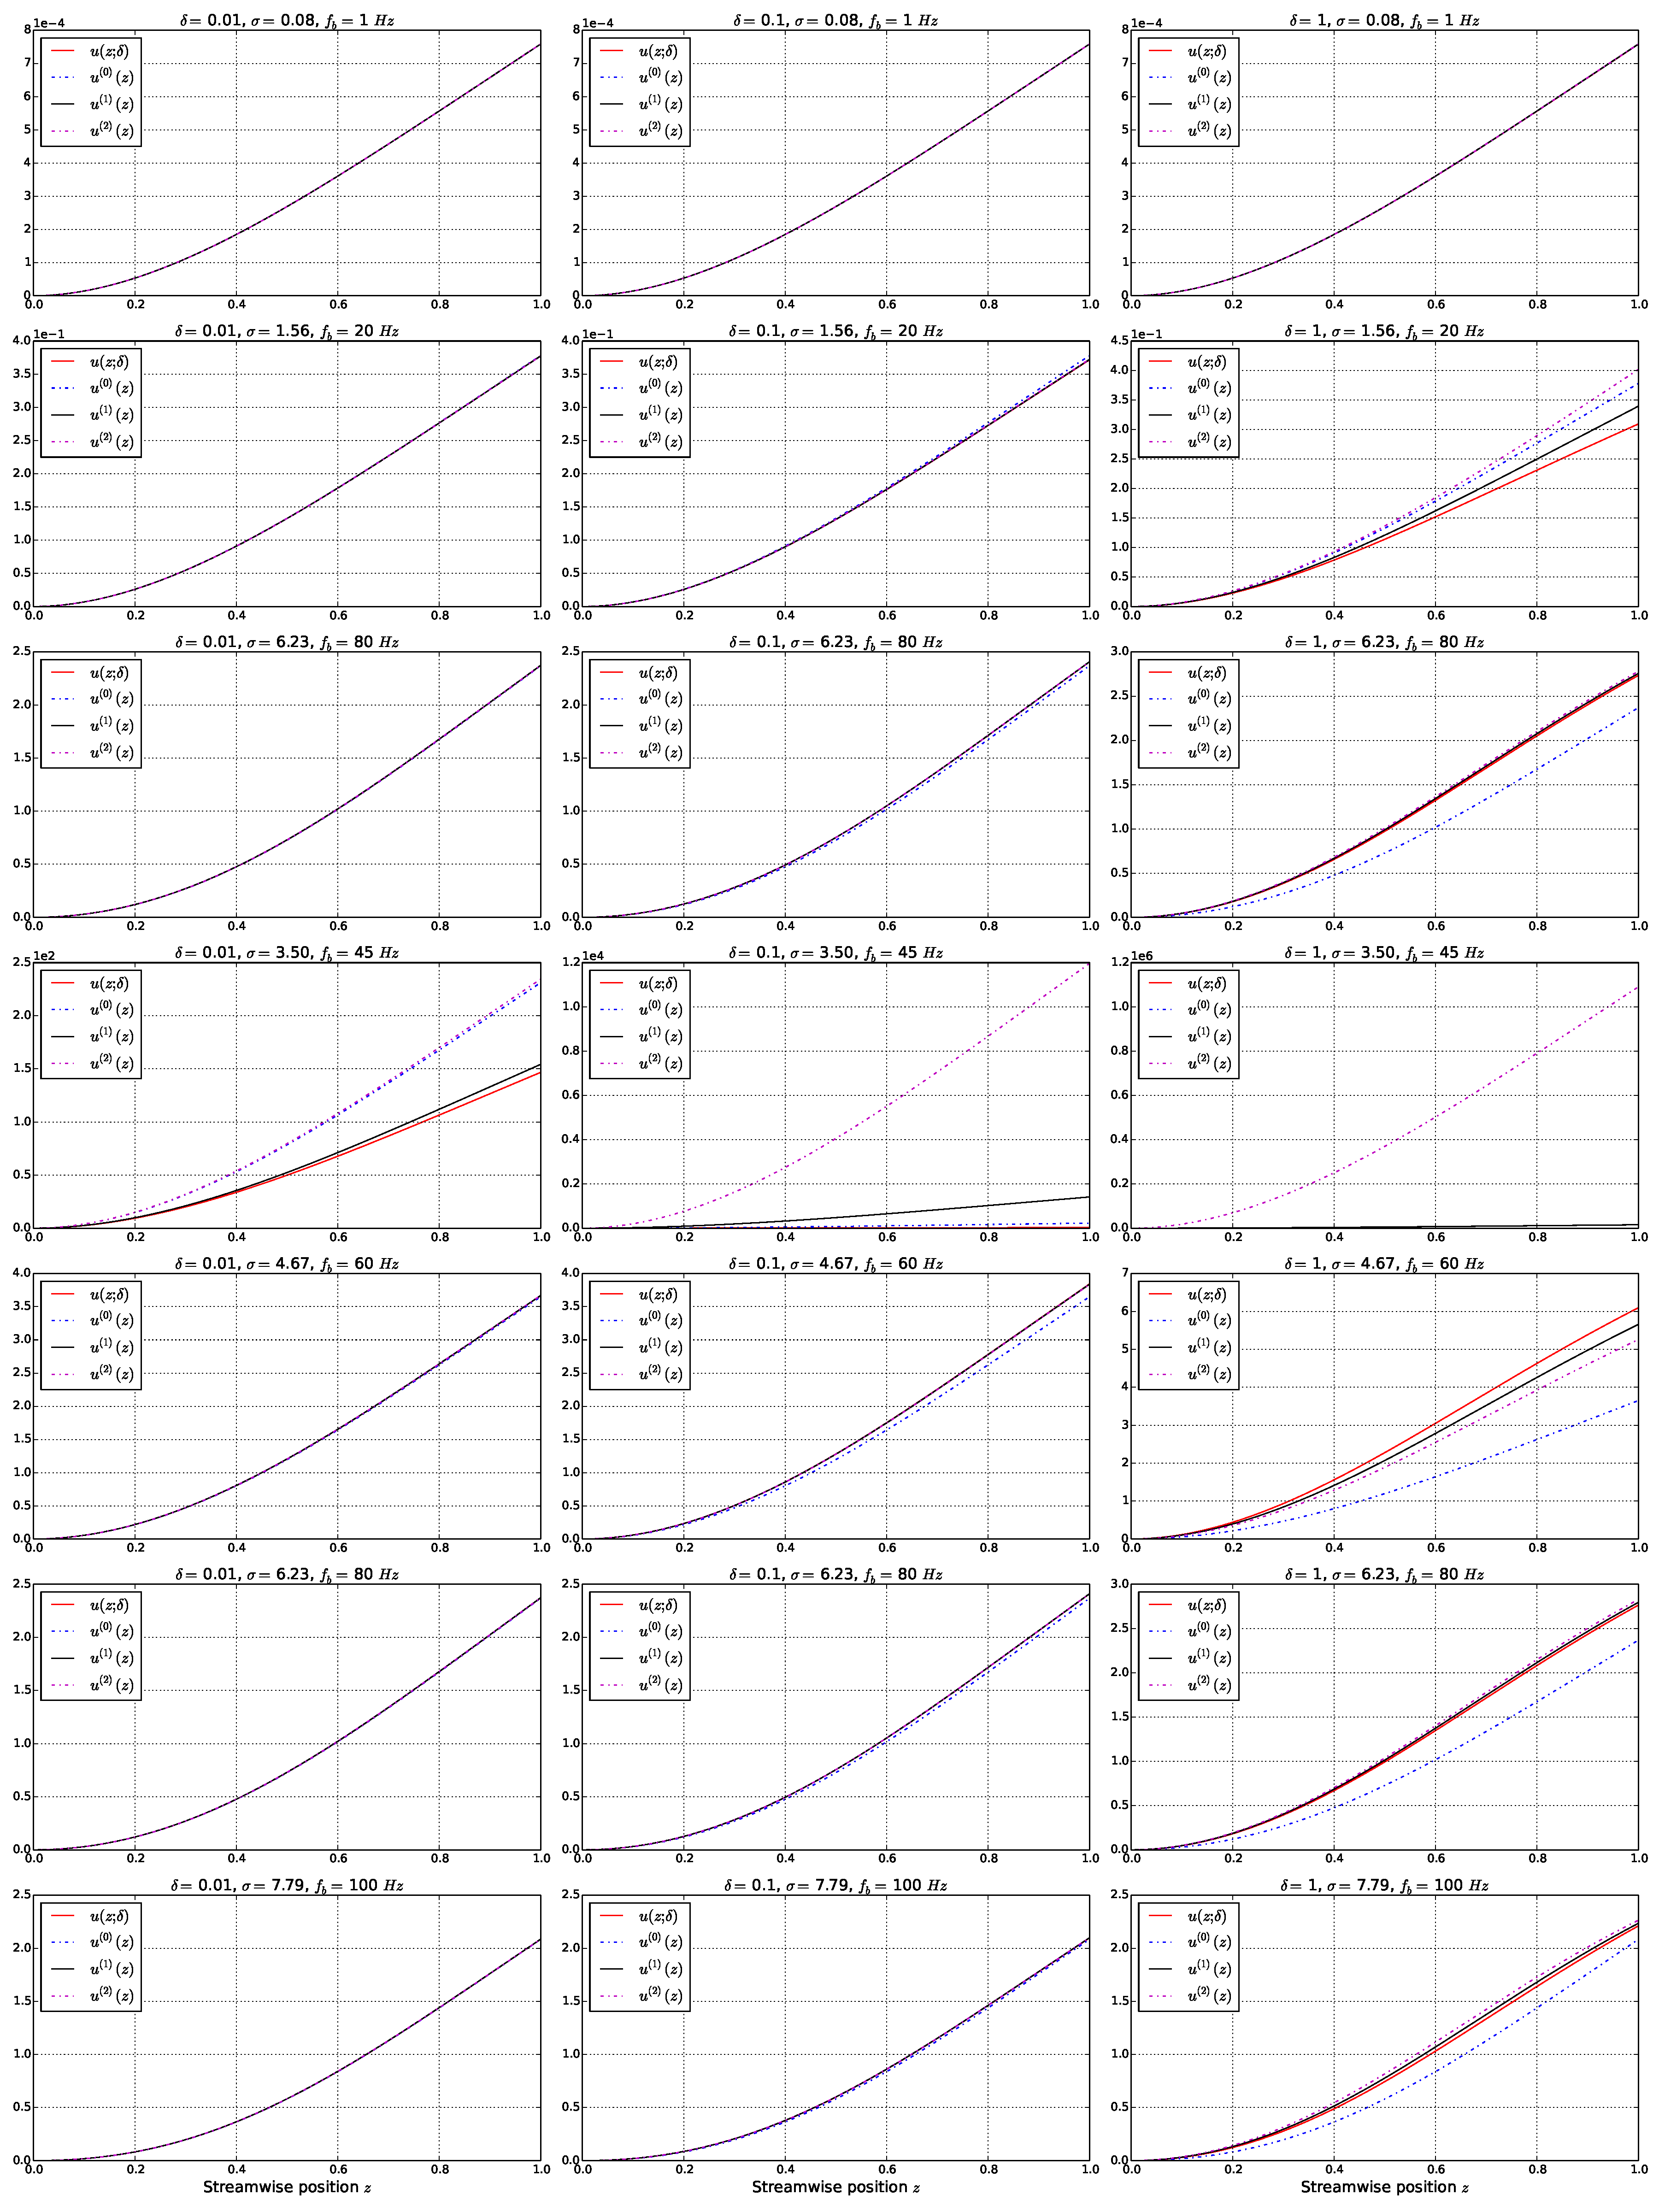
\includegraphics[width=0.8\textwidth]{./img_eig_asy/fig_sol_analytic_disp_cmp_fr_all}
    \caption{Comparison of the asymptotic expansions to different orders for the dimensionless relative displacement function $u(z;\delta)$. The results are calculated at the parameter value of $\beta = 0.064$. The value of $\sigma$ is changed through changing $f_b$. For all the panels in the figure, the horizontal axis denotes the dimensionless streamwise position $z$, and the vertical axis represents the dimensionless relative displacement. }
    \label{fig:fig_sol_analytic_disp_cmp_fr_all}
\end{figure*}


Notice from Figure~\ref{fig:fig_sol_analytic_perf_vs_fr_mod} that the first mode resonant frequency for the PVEH is around $45\ Hz$. It is seen from Figure~\ref{fig:fig_sol_analytic_disp_cmp_fr_all} that generally a smaller value of $\delta$ results in a better approximation, whatever the value of $f_b$. This is consistent with the philosophy behind asymptotic expansion. Besides, for the frequency away from the resonant frequency, the approximation results are relatively accurate in the range of $\delta \leq 0.1$ depending on the value of $f_b$. While the base excitation frequency $f_b$ is close to that of a resonance, for example $f_b = 45\ Hz$, the approximation results are not accurate even at the value of $\delta = 0.01$. That is to say, the asymptotic expansion in terms of $\delta$ is not uniform with respect to parameter $\sigma$. Especially, the existence of resonance actually restricts the performance of the asymptotic expansion. Around the resonance the expansion will show low accuracy, while away from the resonance, the expansion accuracy is easily retained. Nonetheless, for commonly used piezoelectric materials and energy harvesting device configuration, the value of $\delta$ is usually small. Thus the utilization of asymptotic expansion method to approximate the dimensionless relative displacement function $u(z;\delta)$ is to some degree feasible. Furthermore, in view of the approximating performances of the asymptotic expansions to different orders, it suffices to keep only the $0th$ order terms. Then, we have that 
\begin{equation}
    u(z;\delta) \approx u^{(0)}(z) = A_0 \cos{\sqrt{\sigma}z} + B_0 \sin{\sqrt{\sigma}z} + C_0 \cosh{\sqrt{\sigma}z} + D_0 \sinh{\sqrt{\sigma}z} - 1.
\end{equation}
This expression is exactly the relative displacement function of a pure elastic cantilever beam under base excitation. It means that for most piezoelectric energy harvesting devices, due to the fact that the electromechanical coupling factor is relatively small, the relative displacement function is not much affected. In this way, we have indeed uncoupled the electrical part and elastic part of a piezoelectric energy harvesting device. It should be noted that the approximation is not valid near the resonance.


\begin{figure*}[!htbp]
    \centering
    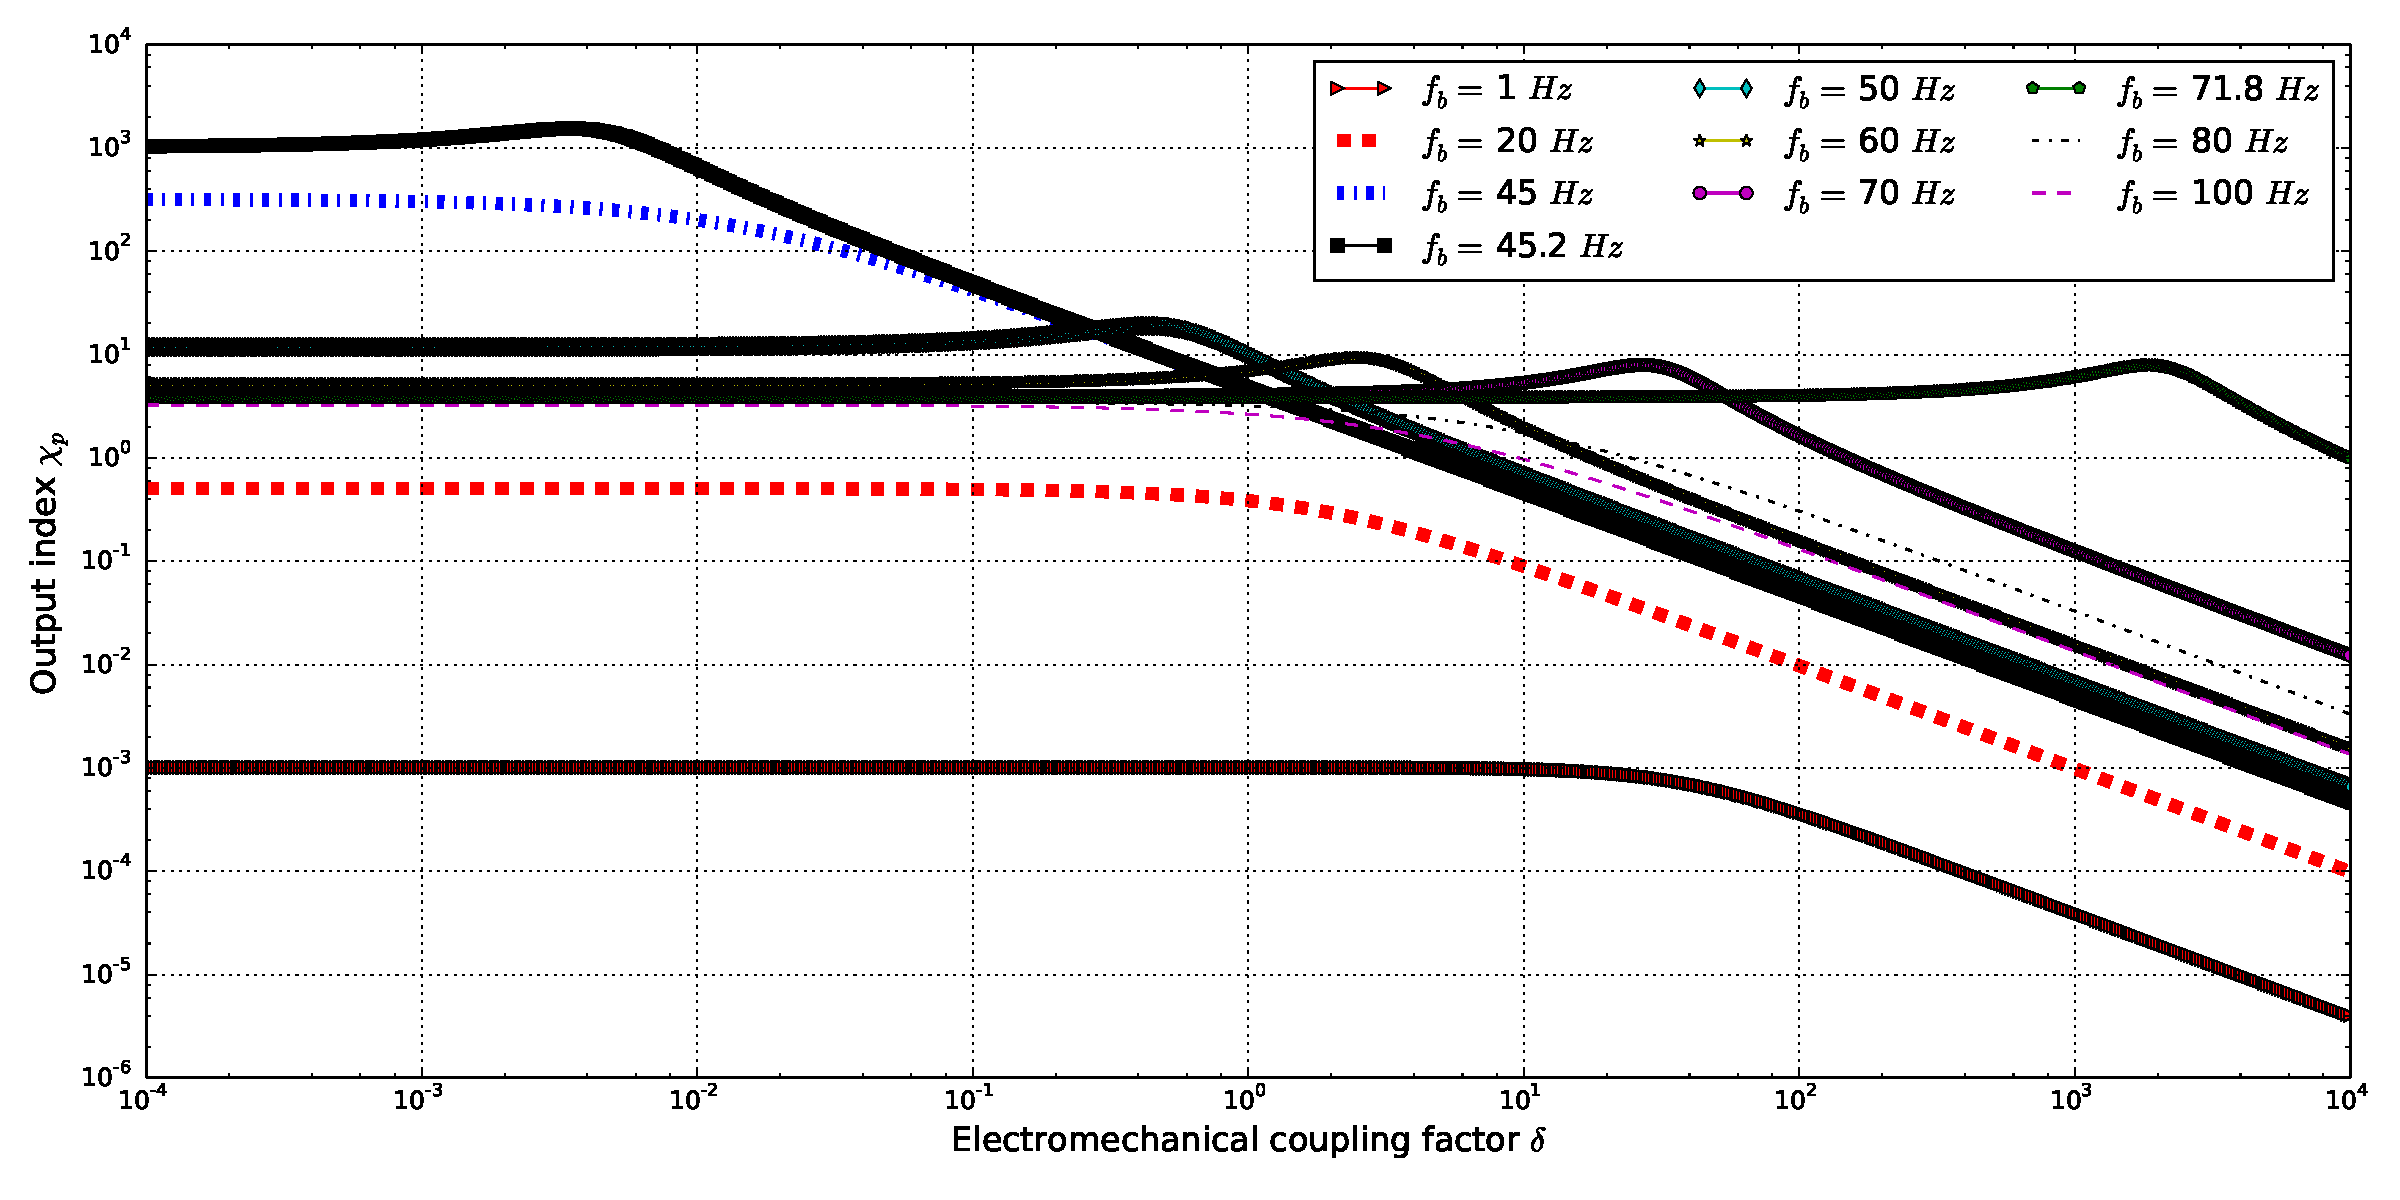
\includegraphics[width=\textwidth]{./img_eig_asy/fig_sol_analytic_out_index_vs_delta}
    \caption{Output index $\chi_p$ as a function of electromechanical coupling factor $\delta$ at different values of base excitation frequency $f_b$. The value of $\beta$ adopted in this simulation is $\beta = 0.321$ corresponding to an external resistance of $R_l = 50\ k\Omega$. }
    \label{fig:fig_sol_analytic_out_index_vs_delta}
\end{figure*}

Furthermore, from equations (\ref{eq:eq_peh_perfs_compact_form}) and (\ref{eq:eq_peh_perfs_compact_form_end_ders}), the output index $\chi_p$ plays a key role in the performance investigation of the PVEH. To see the influences of $\delta$ and $f_b$, therefore $\sigma$, upon $\chi_p$, we firstly calculate the values of $\chi_p$ for different values of $\delta$ by fixing the value of $f_b$ to be some discrete values. The results are shown in Figure~\ref{fig:fig_sol_analytic_out_index_vs_delta}. It is seen that the dependence of $\chi_p$ upon $\delta$ shows two different modes in the frequency range of $1\ \leq f_b \leq \ 100\ Hz$. Firstly, in the frequency range of $45.2\ Hz \leq f_b \leq 71.8\ Hz$, a peak value of output index $\chi_p$ is reached at a critical value of $\delta = \delta_p^{(c)}$. When $\delta$ is smaller than $\delta_p^{(c)}$, the output index $\chi_p$ increases along with $\delta$, and when $\delta$ is larger than $\delta_p^{(c)}$, the output index $\chi_p$ decreases with the increase of $\delta$. It should be noted that the limit values of the frequency range discussed here are not strictly accurate as a result of the selection of numerical computation grids. Secondly, for the frequency range of $f_b \leq 45\ Hz$ or $f_b \geq 80\ Hz$, the output index $\chi_p$ shows a monotonic decrease with respect to the increase $\delta$.


\begin{figure*}[!htbp]
    \centering
    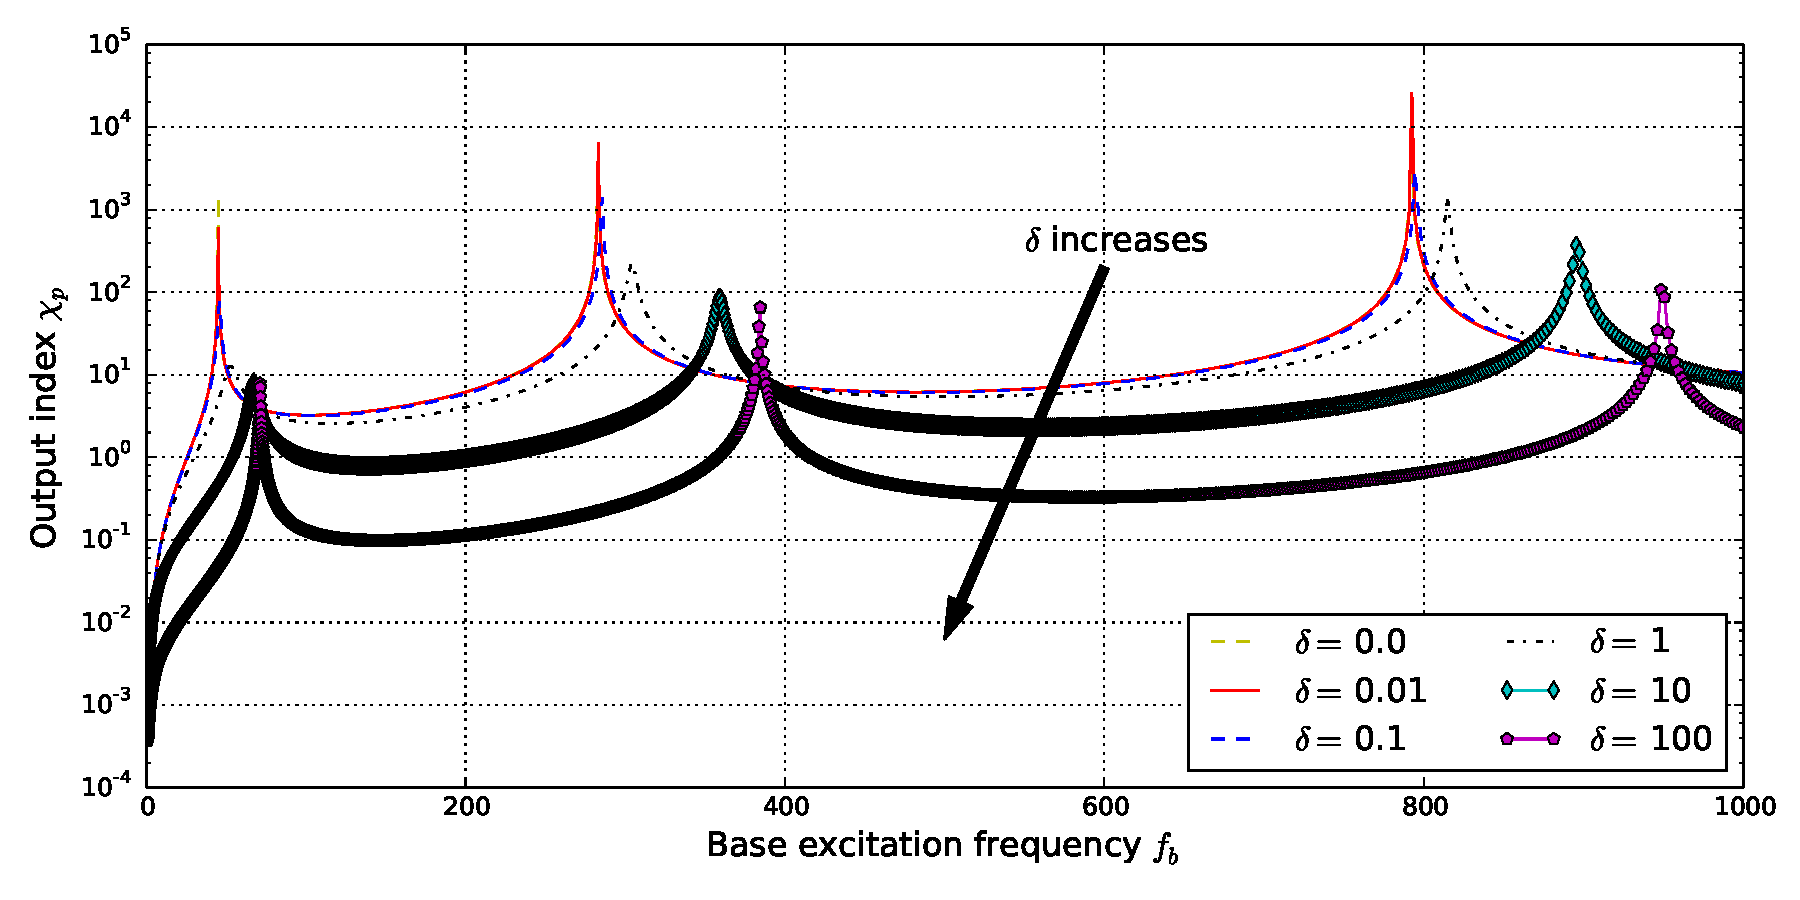
\includegraphics[width=\textwidth]{./img_eig_asy/fig_sol_analytic_out_index_vs_fr}
    \caption{Output index $\chi_p$ as a function of base excitation frequency $f_b$ at different values of electromechanical coupling factor $\delta$. The value of $\beta$ adopted in this simulation is $\beta = 0.321$ corresponding to an external resistance of $R_l = 50\ k\Omega$. }
    \label{fig:fig_sol_analytic_out_index_vs_fr}
\end{figure*}


Alternatively, by fixing the values of $\delta$ to a discrete set of numbers, we calculate the values of $\chi_p$ in relation to different values of $f_b$. This is very similar to a frequency response of the output index as a function of $\sigma$. The results are shown in Figure~\ref{fig:fig_sol_analytic_out_index_vs_fr}. It is shown that with the increase of electromechanical coupling factor $\delta$, the resonant frequencies to the system increase with the increase of $\delta$. This is indicated by the shift to the right of the frequency response curve of output index $\chi_p$. Besides, we add in this figure the case where $\delta = 0.0$ as a reference. Simple comparisons show that the discrepancy between the frequency response curves of $\chi_p$ related to the case of $\delta = 0$, $\delta=0.01$, and $\delta = 0.1$ is small. A direct conclusion can be made that for small values of electromechanical coupling factor $\delta$, the output index $\chi_p$ can be approximated by 
\begin{equation}
    \chi_p \approx \frac{ \sqrt{\sigma} \left( \sinh\sqrt{\sigma} - \sin\sqrt{\sigma} \right) }{ 1 + \cos\sqrt{\sigma } \cosh\sqrt{\sigma } }.
\end{equation}
which is actually consistent with the above presented asymptotic expansion process. As a result, the output performance measures $\tilde{V}_p$, $\tilde{I}_p$, and $\tilde{P}_p$ can be approximated by 
\begin{equation}
    \left\{\begin{aligned}
        \tilde{V}_p &= - \frac{j \sigma \beta}{j \sigma \beta + 1} \left(\frac{\eta_b}{l_p}\right) \left(\frac{e_p}{C_p}\right) \frac{ \sqrt{\sigma} \left( \sinh\sqrt{\sigma} - \sin\sqrt{\sigma} \right) }{ 1 + \cos\sqrt{\sigma } \cosh\sqrt{\sigma } } , \\
        \tilde{I}_p &= - \frac{ j \sigma \beta } {j \sigma \beta + 1} \left( \frac{\eta_b}{l_p} \right) \left( \frac{e_p}{C_p R_l} \right) \frac{ \sqrt{\sigma} \left( \sinh\sqrt{\sigma} - \sin\sqrt{\sigma} \right) }{ 1 + \cos\sqrt{\sigma } \cosh\sqrt{\sigma } }, \\
        \tilde{P}_p &= \left(\frac{\eta_b}{l_p}\right)^2 \left(\frac{e_p}{C_p}\right) \left( \frac{e_p}{C_p R_l} \right) \left( \frac{ j \sigma \beta}{ j \sigma \beta + 1 } \right)^2 \left( \frac{ \sqrt{\sigma} \left( \sinh\sqrt{\sigma} - \sin\sqrt{\sigma} \right) }{ 1 + \cos\sqrt{\sigma } \cosh\sqrt{\sigma } } \right)^2.
    \end{aligned}\right.
    \label{eq:eq_peh_perfs_compact_form_approx}
\end{equation}




\begin{figure*}[!htbp]
    \centering
    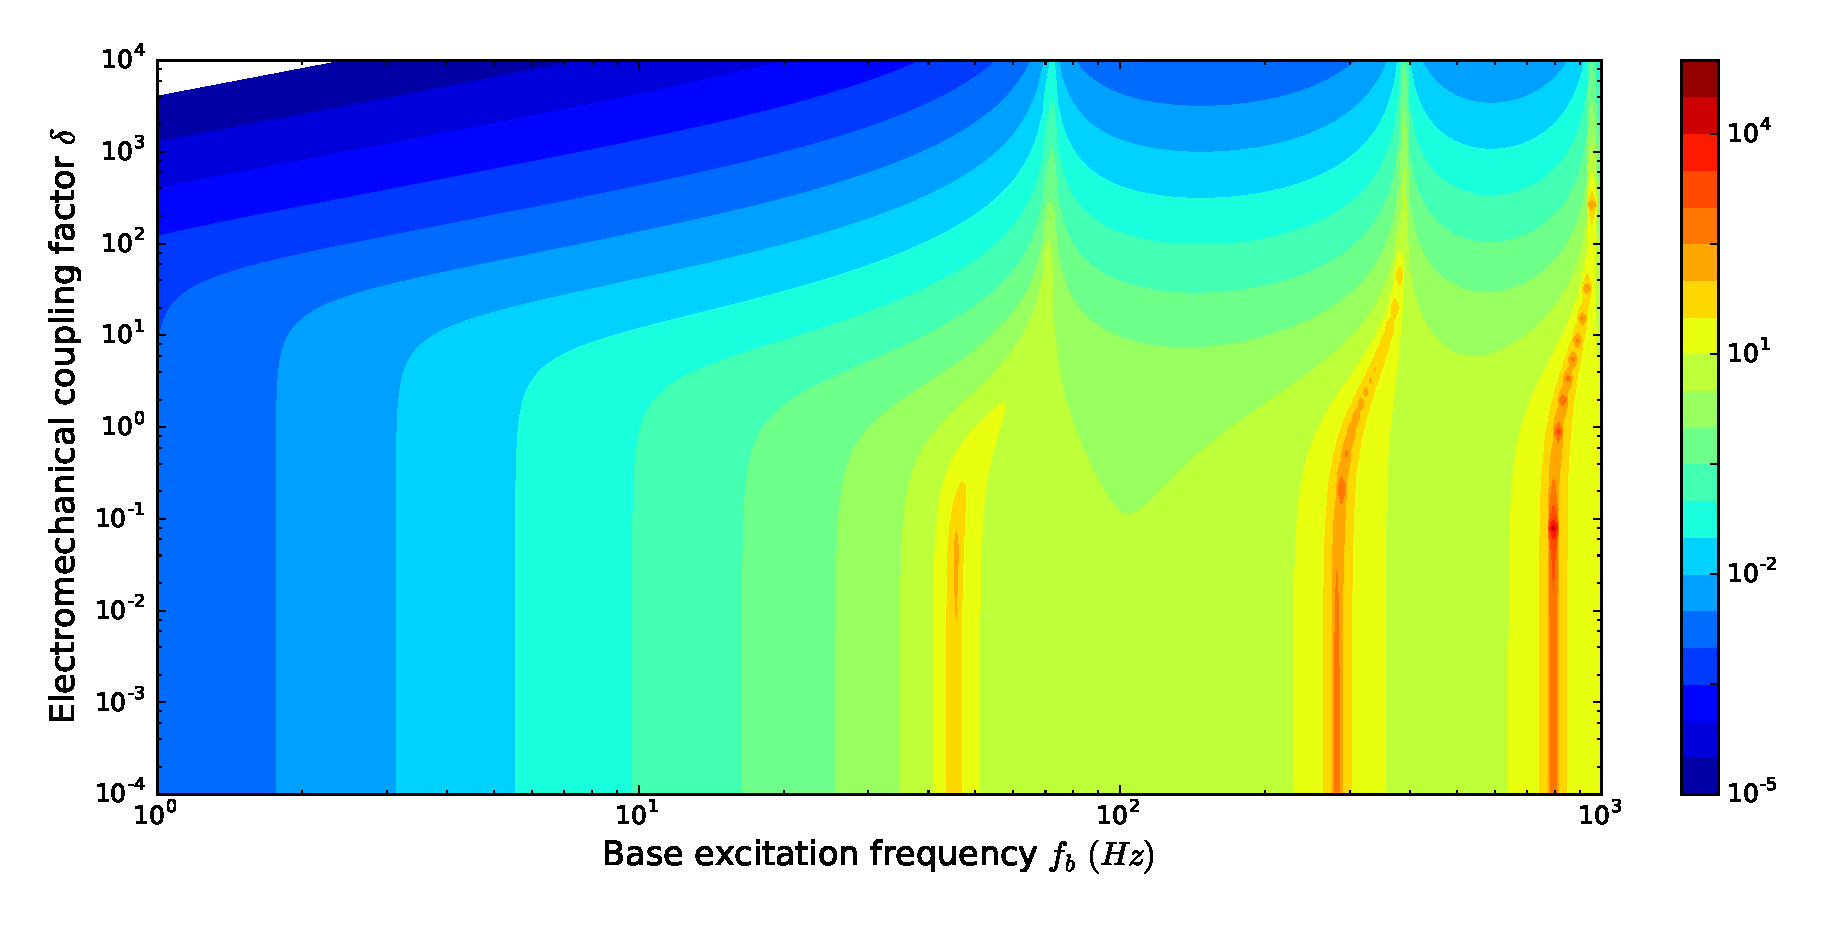
\includegraphics[width=\textwidth]{./img_eig_asy/fig_sol_analytic_out_index_contour}
    \caption{Output index $\chi_p$ as a function of base excitation frequency $f_b$ and electromechanical coupling factor $\delta$. The value of $\beta$ adopted in this simulation is $\beta = 0.321$ corresponding to an external resistance of $R_l = 50\ k\Omega$. }
    \label{fig:fig_sol_analytic_out_index_contour}
\end{figure*}

Furthermore, a closer look into the synergistic influence of the two parameters $\sigma$ and $\delta$ upon the output index $\chi_p$, the output voltage amplitude $\tilde{V}_p$, and the output power amplitude $\tilde{P}_p$ is taken. The output index $\chi_p$ as a function of $\sigma$ (hence $f_b$) and $\delta$ is plotted in Figure~\ref{fig:fig_sol_analytic_out_index_contour}, while the output voltage amplitude $\tilde{V}_p$ and the output power amplitude $\tilde{P}_p$ as functions of $\sigma$ (hence $f_b$) and $\delta$ are plotted in Figure~\ref{fig:fig_sol_analytic_out_vol_contour} and Figure~\ref{fig:fig_sol_analytic_out_pow_contour} respectively.

\begin{figure*}[!htbp]
    \centering
    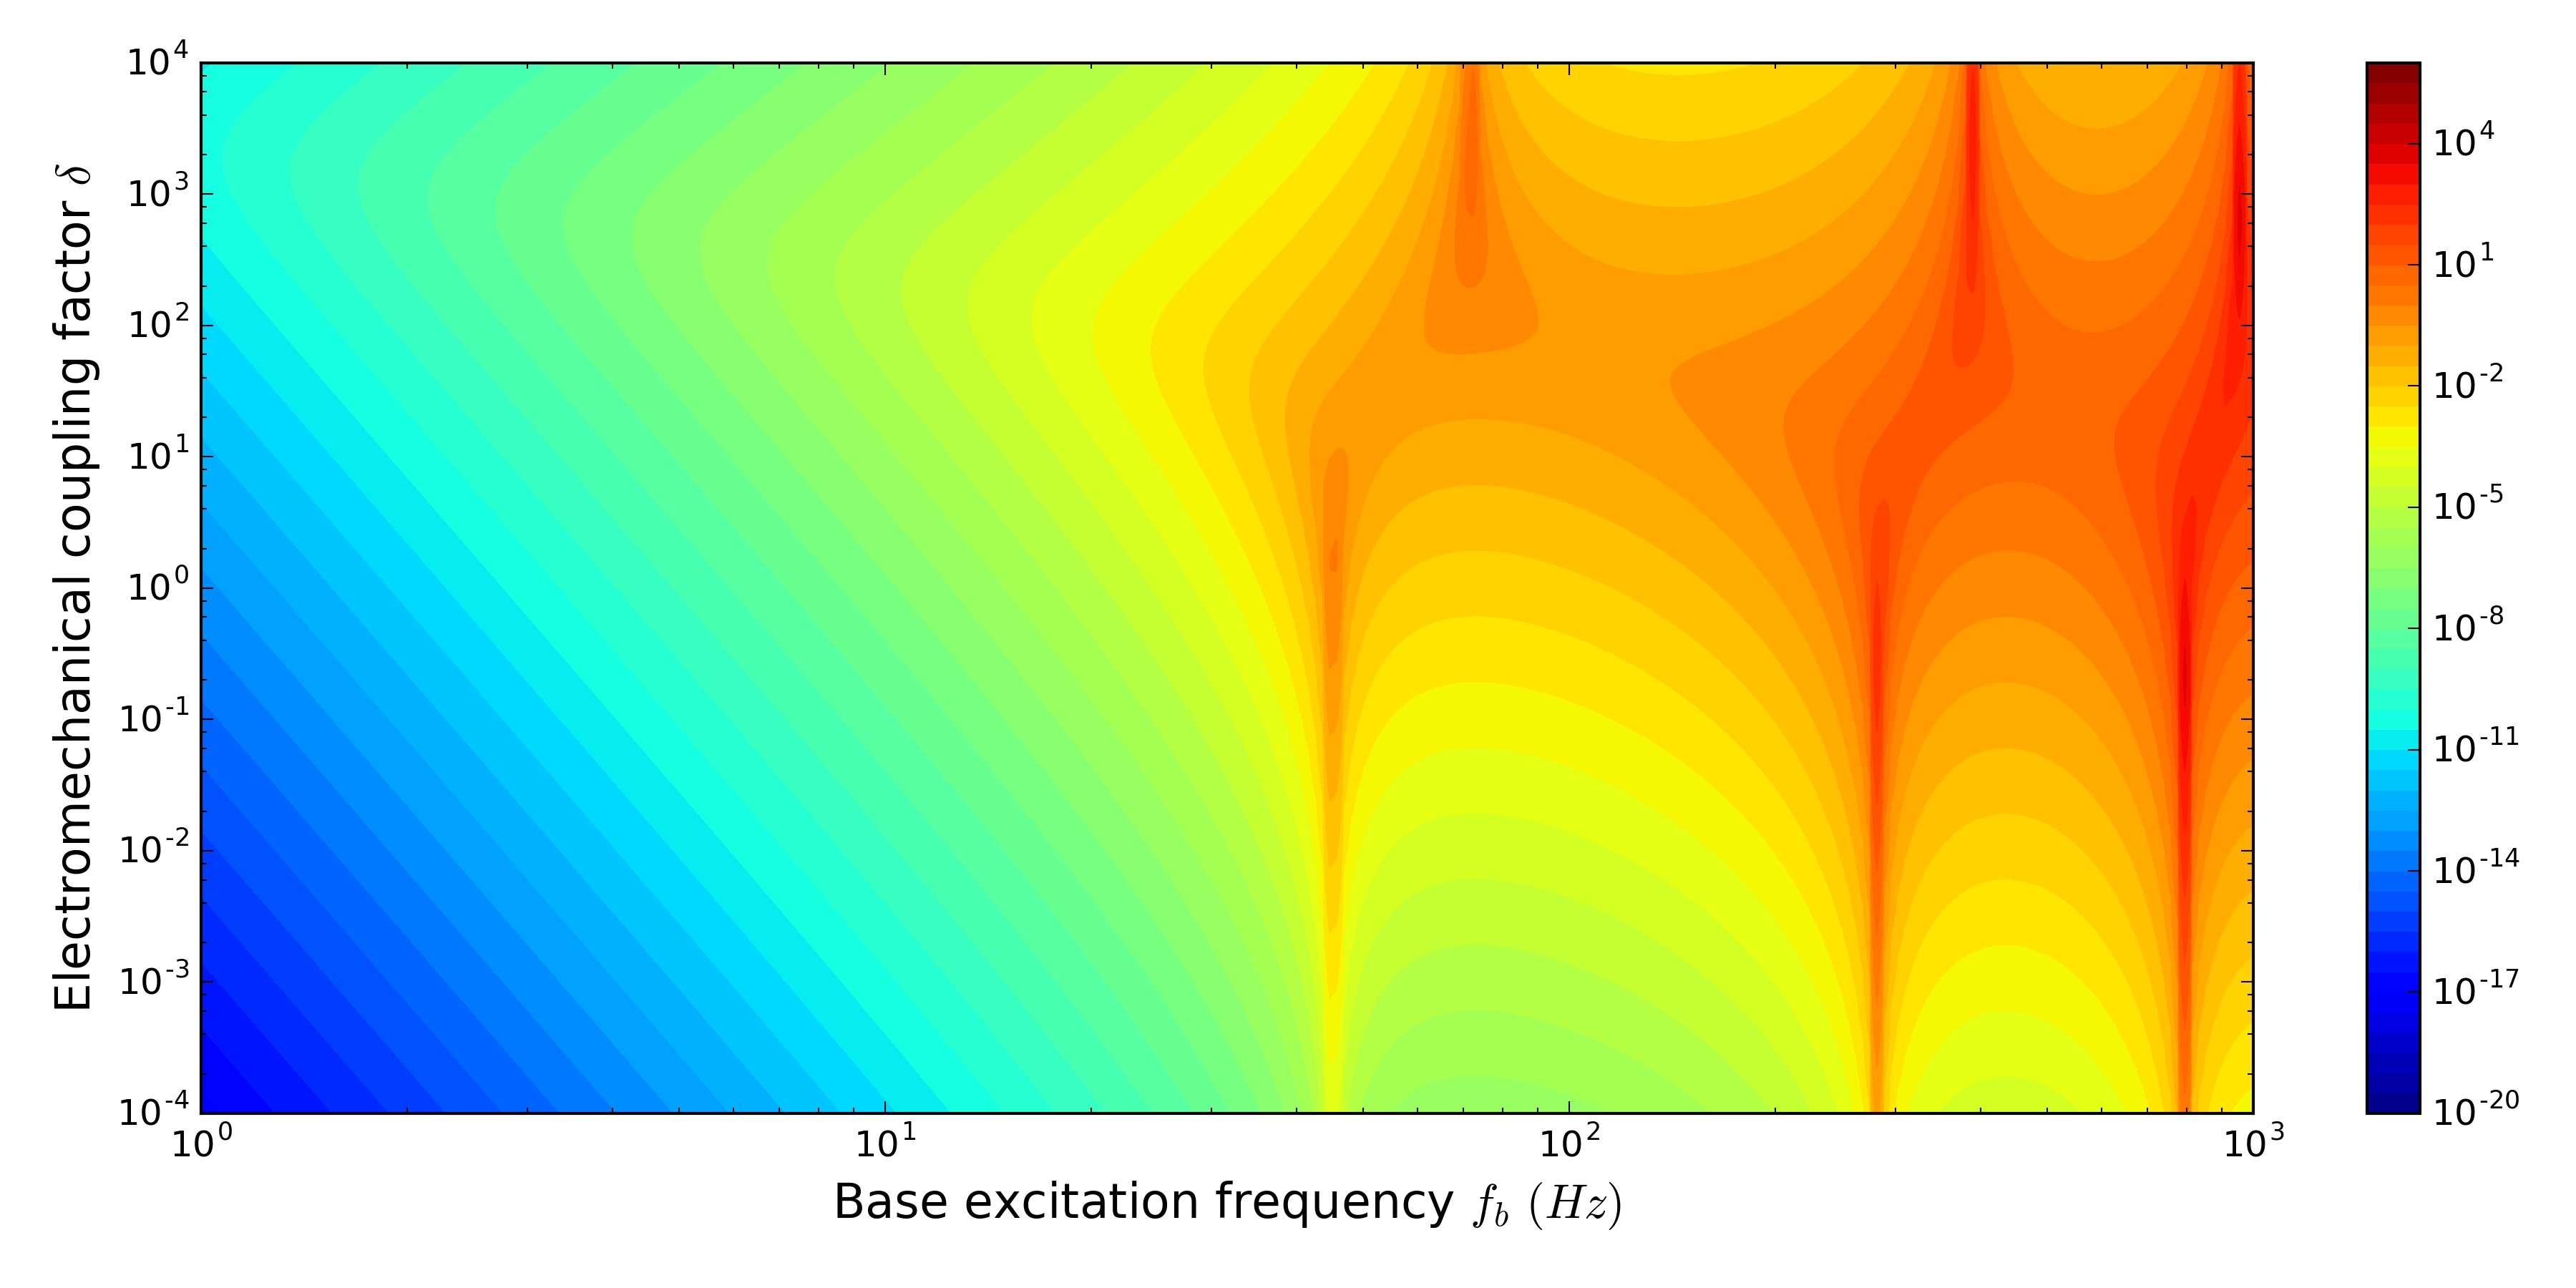
\includegraphics[width=\textwidth]{./img_eig_asy/fig_sol_analytic_out_vol_contour}
    \caption{Output voltage amplitude $\tilde{V}_p$ as a function of base excitation frequency $f_b$ and electromechanical coupling factor $\delta$. In the simulations a load resistance of $R_l = 1\ k\Omega$ is adopted.}
    \label{fig:fig_sol_analytic_out_vol_contour}
\end{figure*}

\begin{figure*}[!htbp]
    \centering
    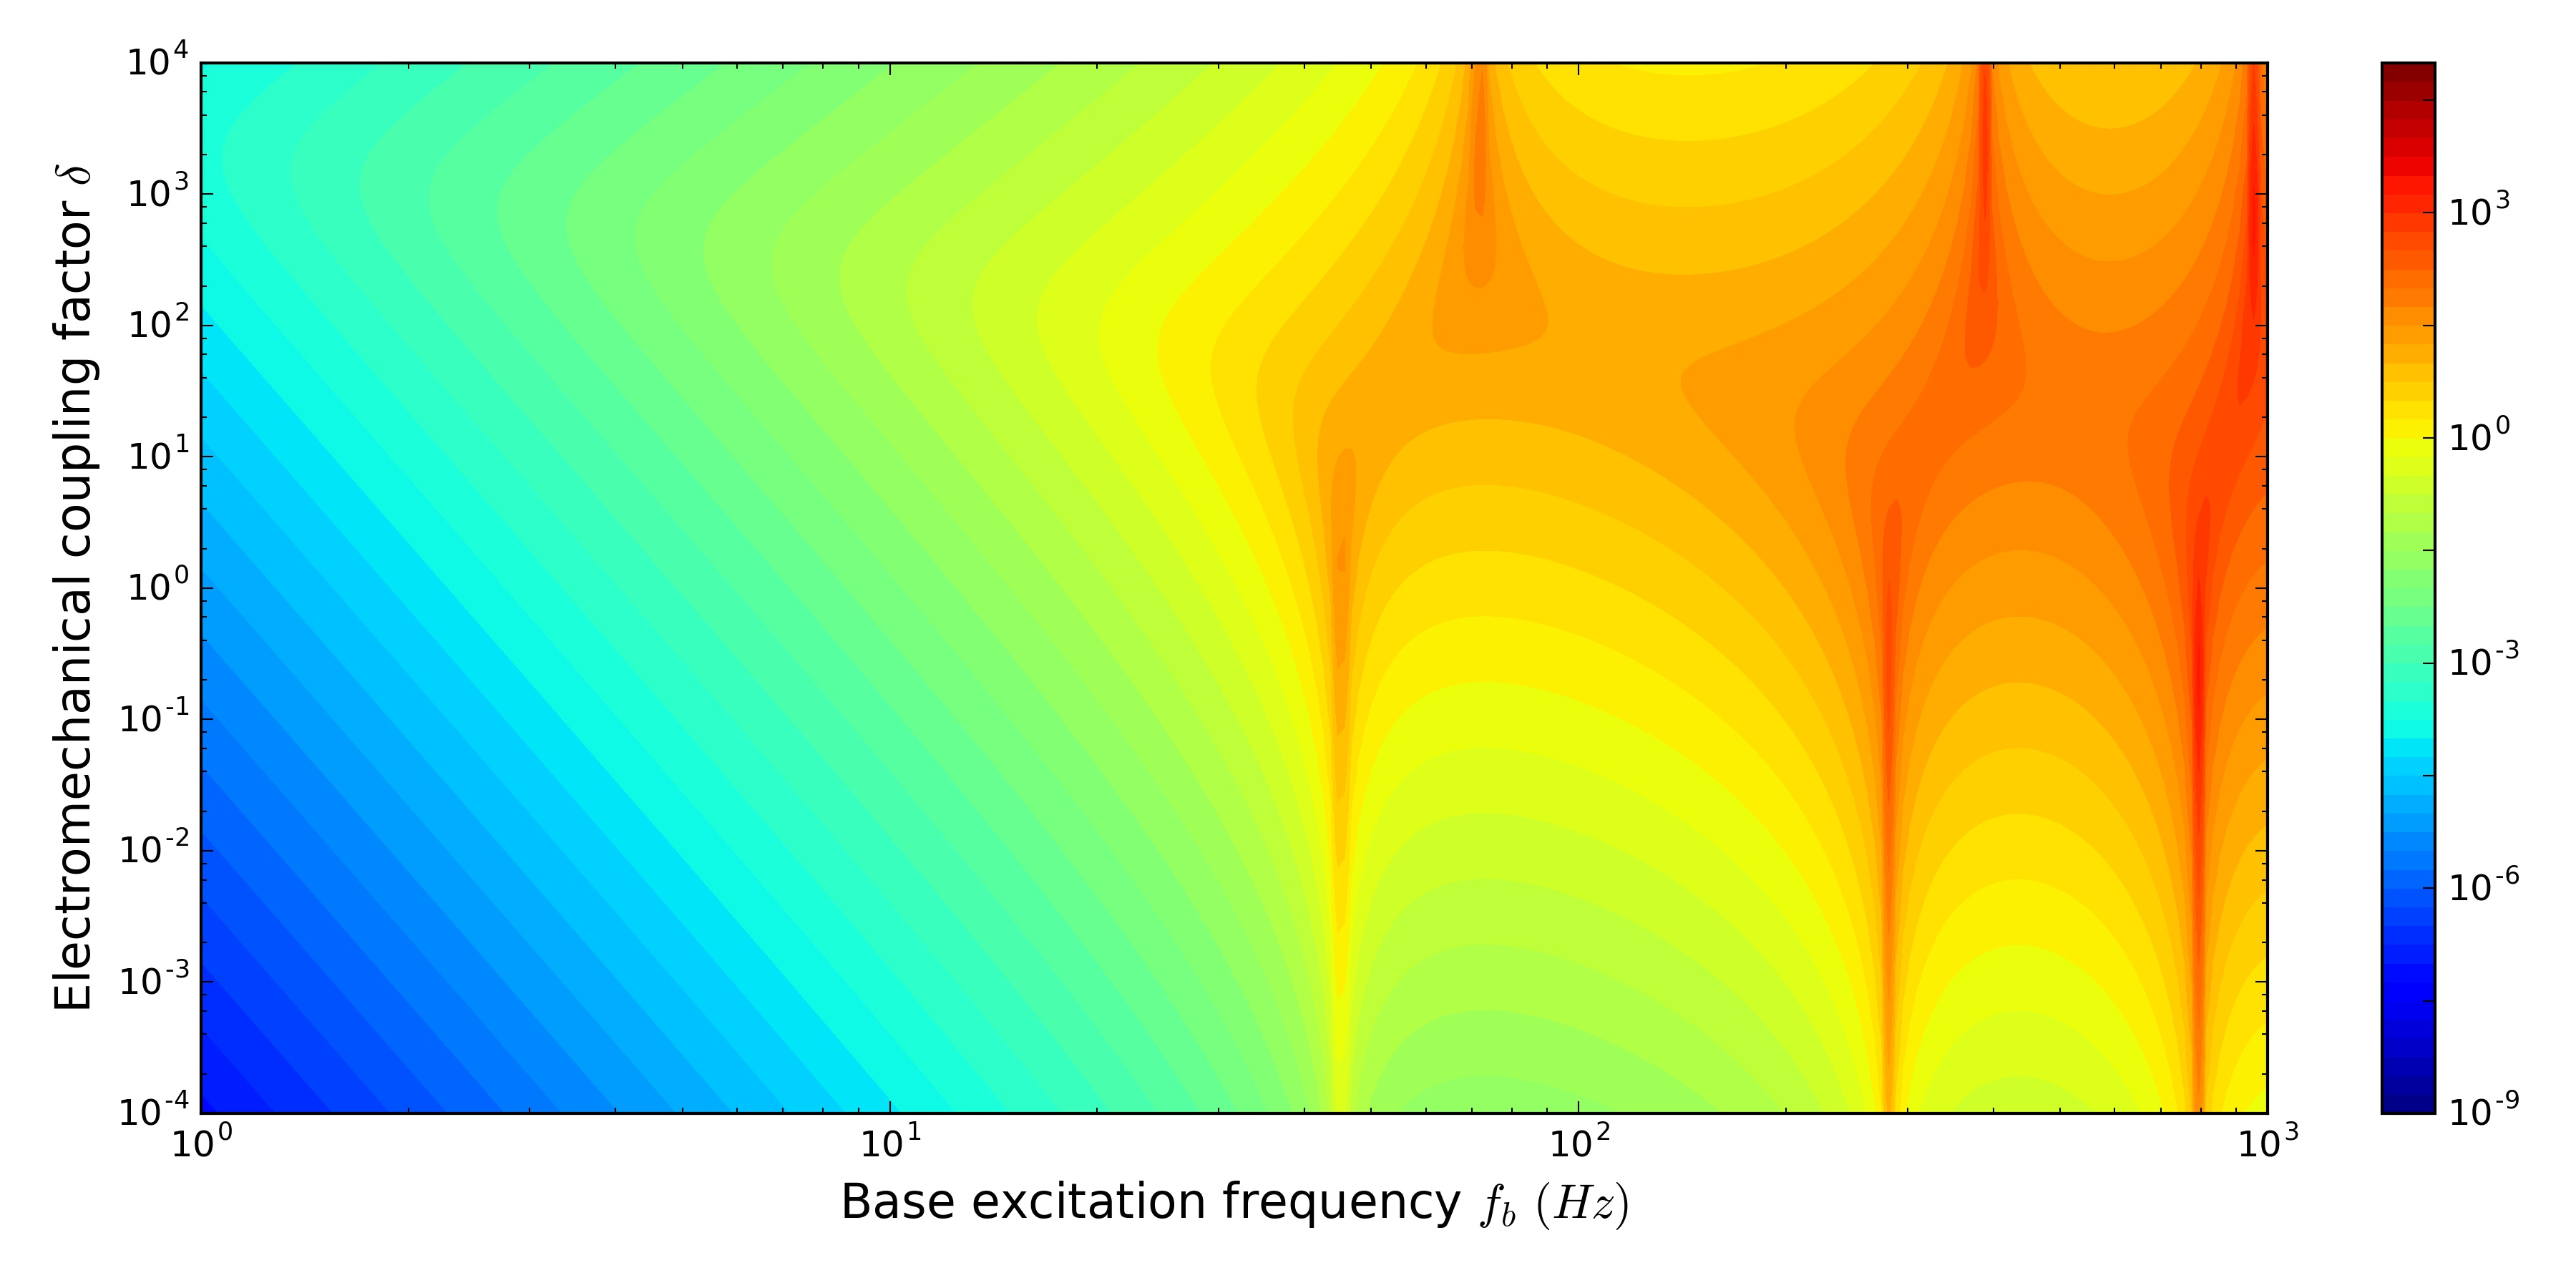
\includegraphics[width=\textwidth]{./img_eig_asy/fig_sol_analytic_out_pow_contour}
    \caption{ Output power amplitude $\tilde{P}_p$ as a function of base excitation frequency $f_b$ and electromechanical coupling factor $\delta$. In the simulations a load resistance of $R_l = 1\ k\Omega$ is adopted.}
    \label{fig:fig_sol_analytic_out_pow_contour}
\end{figure*}


According to Figure~\ref{fig:fig_sol_analytic_out_index_contour}, Figure~\ref{fig:fig_sol_analytic_out_vol_contour} and Figure~\ref{fig:fig_sol_analytic_out_pow_contour}, three narrow peak regions are present in the range of parameters considered, whatever the performance measures chosen. There can be large change in the order of magnitude for the performance measures when the parameter values are slightly away from the peak regions. Another point can be extracted that the increase of electromechanical coupling factor $\delta$ does not always leads to an increase of the output performances. For some value of $f_b$, a larger $\delta$ necessarily determines a larger output, while for some other values of $f_b$ a smaller value of $\delta$ is preferential. What's more, for some specific values of $\delta$, an intermediate value of $\delta$ is expected for a better output performance. Hence, to obtain a better energy harvesting performance for the PVEH, the frequency range should be considered along with the electromechanical coupling factor of the energy harvester designed. Future focus should be made upon the matching and optimization of the parameter values in a designed PVEH.


\section{Conclusion}

Piezoelectric vibration energy harvesting has attracted much research attention with the prospect of fully or completely replacing batteries for low-power electronics. Models of PVEHs are of key importance in the design and optimization of piezoelectric energy harvesters. In this contribution, we put forward a new way to theoretically express the solution to the base excitation problem of a PVEH. Analytical expressions of the solutions are given with validations done with respect to the currently adopted solutions. Asymptotic expansion analysis are then conducted to obtain the approximations of the dimensionless relative displacement function and the corresponding output index and output performance measures. Tips for design and optimization of piezoelectric energy harvesters are given. 

\section*{Appendix}
\label{sec:sec_appendix}

\begin{equation}
    \left\{\begin{aligned}
        A_{k+1} + C_{k+1} &= 0, \\
        B_{k+1} + D_{k+1} &= 0, \\
        \left( - A_{k+1} \cos{\sqrt{\sigma}} - B_{k+1} \sin{\sqrt{\sigma}} + C_{k+1} \cosh{\sqrt{\sigma}} + D_{k+1} \sinh{\sqrt{\sigma}} \right) &+ \\
        \frac{j \beta \sqrt{\sigma}}{ j\sigma \beta + 1 } \left( - A_{k} \sin{\sqrt{\sigma}} + B_{k} \cos{\sqrt{\sigma}} + C_{k} \sinh{\sqrt{\sigma}} + D_{k} \cosh{\sqrt{\sigma}} \right) &= 0, \\
        A_{k+1} \sin{\sqrt{\sigma}} - B_{k+1} \cos{\sqrt{\sigma}} + C_{k+1} \sinh{\sqrt{\sigma}} + D_{k+1} \cosh{\sqrt{\sigma}} &= 0,
    \end{aligned}\right.
\end{equation}
whose solution is expressed by
\begin{equation}
    \left\{\begin{aligned}
        A_{k+1} &= \left( \frac{j \beta \sqrt{\sigma }}{1+j \beta \sigma } \right) \left(\frac{\cos\sqrt{\sigma }+\cosh\sqrt{\sigma }}{2 \cos\sqrt{\sigma }\cosh\sqrt{\sigma }+2} \right) \left( Q_k \right), \\
        B_{k+1} &= \left( \frac{j \beta \sqrt{\sigma }}{1+j \beta \sigma } \right) \left( \frac{-\sinh\sqrt{\sigma }+\sin\sqrt{\sigma }}{2 \cos\sqrt{\sigma }\cosh\sqrt{\sigma }+2} \right) \left( Q_k \right), \\
        C_{k+1} &= \left( \frac{j \beta \sqrt{\sigma }}{1+j \beta \sigma } \right) \left( -\frac{\cos\sqrt{\sigma }+\cosh\sqrt{\sigma }}{2 \cos\sqrt{\sigma } \cosh\sqrt{\sigma }+2} \right) \left( Q_k \right), \\
        D_{k+1} &= \left( \frac{j \beta \sqrt{\sigma }}{1+j \beta \sigma } \right) \left( \frac{-\sin\sqrt{\sigma }+\sinh\sqrt{\sigma }}{2 \cos\sqrt{\sigma }\cosh\sqrt{\sigma }+2} \right) \left( Q_k \right), 
    \end{aligned}\right.
\end{equation}
in which
\begin{equation}
    Q_k = - A_{k} \sin{\sqrt{\sigma}} + B_{k} \cos{\sqrt{\sigma}} + C_{k} \sinh{\sqrt{\sigma}} + D_{k} \cosh{\sqrt{\sigma}}.
\end{equation}


In terms of $Q_k$ ($k \geq 0$), we have the following iterative relation
\begin{equation}
    Q_{k+1} = - \left( \frac{ \sin\sqrt{\sigma} \cosh\sqrt{\sigma} + \cos\sqrt{\sigma} \sinh\sqrt{\sigma} }{ \cos\sqrt{\sigma }\cosh\sqrt{\sigma }+1 } \right) \left( \frac{j \beta \sqrt{\sigma }}{1+j \beta \sigma } \right) Q_k,
\end{equation}
and the initial two values $Q_0$ and $Q_1$:
\begin{equation}
    \left\{\begin{aligned}
        Q_0 &= \frac{\sinh\sqrt{\sigma }-\sin\sqrt{\sigma }}{\cos\sqrt{\sigma } \cosh\sqrt{\sigma }+1}, \\
        Q_{1} &= \frac{j \beta  \sqrt{\sigma }}{1+j \beta  \sigma } \left(\frac{\sin\sqrt{\sigma } -\sinh\sqrt{\sigma }}{\cos\sqrt{\sigma } \cosh\sqrt{\sigma }+1} \right)  \left( \frac{\cos\sqrt{\sigma } \sinh\sqrt{\sigma }+\sin\sqrt{\sigma } \cosh\sqrt{\sigma }}{\cos\sqrt{\sigma } \cosh\sqrt{\sigma }+1} \right).
    \end{aligned}\right.
\end{equation}
Hence it is shown that for $k \geq 0$,
\begin{equation}
    Q_{k} = \left[- \left( \frac{j \beta \sqrt{\sigma }}{1+j \beta \sigma } \right) \left( \frac{ \sin\sqrt{\sigma} \cosh\sqrt{\sigma} + \cos\sqrt{\sigma} \sinh\sqrt{\sigma} }{ \cos\sqrt{\sigma }\cosh\sqrt{\sigma }+1 } \right)  \right]^k \left( \frac{\sinh\sqrt{\sigma }-\sin\sqrt{\sigma }}{\cos\sqrt{\sigma } \cosh\sqrt{\sigma }+1} \right).
\end{equation}
As a result, we obtain that for $k \geq 1$,
\footnotesize
\begin{equation*}
    \left\{\begin{aligned}
        A_{k} &= \left( \frac{j \beta \sqrt{\sigma }}{1+j \beta \sigma } \right)^{k} \left( \frac{ -\sin\sqrt{\sigma} \cosh\sqrt{\sigma} - \cos\sqrt{\sigma} \sinh\sqrt{\sigma} }{ \cos\sqrt{\sigma }\cosh\sqrt{\sigma }+1 } \right)^{k-1} \left( \frac{\sinh\sqrt{\sigma }-\sin\sqrt{\sigma }}{\cos\sqrt{\sigma } \cosh\sqrt{\sigma }+1} \right) \left(\frac{\cos\sqrt{\sigma }+\cosh\sqrt{\sigma }}{2 \cos\sqrt{\sigma }\cosh\sqrt{\sigma }+2} \right), \\
        B_{k} &= \left( \frac{j \beta \sqrt{\sigma }}{1+j \beta \sigma } \right)^{k}  \left( \frac{ -\sin\sqrt{\sigma} \cosh\sqrt{\sigma} - \cos\sqrt{\sigma} \sinh\sqrt{\sigma} }{ \cos\sqrt{\sigma }\cosh\sqrt{\sigma }+1 } \right)^{k-1} \left( \frac{\sinh\sqrt{\sigma }-\sin\sqrt{\sigma }}{\cos\sqrt{\sigma } \cosh\sqrt{\sigma }+1} \right) \left( \frac{-\sinh\sqrt{\sigma }+\sin\sqrt{\sigma }}{2 \cos\sqrt{\sigma }\cosh\sqrt{\sigma }+2} \right), \\
        C_{k} &= \left( \frac{j \beta \sqrt{\sigma }}{1+j \beta \sigma } \right)^{k}  \left( \frac{ -\sin\sqrt{\sigma} \cosh\sqrt{\sigma} - \cos\sqrt{\sigma} \sinh\sqrt{\sigma} }{ \cos\sqrt{\sigma }\cosh\sqrt{\sigma }+1 } \right)^{k-1} \left( \frac{\sinh\sqrt{\sigma }-\sin\sqrt{\sigma }}{\cos\sqrt{\sigma } \cosh\sqrt{\sigma }+1} \right) \left( \frac{-\cos\sqrt{\sigma }-\cosh\sqrt{\sigma }}{2 \cos\sqrt{\sigma } \cosh\sqrt{\sigma }+2} \right), \\
        D_{k} &= \left( \frac{j \beta \sqrt{\sigma }}{1+j \beta \sigma } \right)^{k} \left( \frac{ -\sin\sqrt{\sigma} \cosh\sqrt{\sigma} - \cos\sqrt{\sigma} \sinh\sqrt{\sigma} }{ \cos\sqrt{\sigma }\cosh\sqrt{\sigma }+1 } \right)^{k-1} \left( \frac{\sinh\sqrt{\sigma }-\sin\sqrt{\sigma }}{\cos\sqrt{\sigma } \cosh\sqrt{\sigma }+1} \right) \left( \frac{-\sin\sqrt{\sigma }+\sinh\sqrt{\sigma }}{2 \cos\sqrt{\sigma }\cosh\sqrt{\sigma }+2} \right).
    \end{aligned}\right.
\end{equation*}
\normalsize



\section*{Acknowledgments}
The authors would like to thank the financial support from the National Natural Science Foundation of China (NSFC) under contract number 51705112. The research presented in this paper is also supported by the Zhejiang Provincial Natural Science Foundation of China under Grant No. LQ18E050007.

\bibliography{analysis_eig_asy.bib}
\bibliographystyle{vancouver}


\end{document}
% end of file template.tex

